\documentclass{article}
\usepackage[utf8]{inputenc}
\usepackage[top=3cm,bottom=3cm,left=2cm,right=2cm]{geometry}
\usepackage{natbib}
\usepackage{graphicx}
\usepackage{amsmath}
\usepackage{amssymb}
\usepackage{amsthm}
\usepackage{amsfonts}
\usepackage{hyperref}
\usepackage{xcolor}
\usepackage{titlesec}
\usepackage{ifthen,tabto}
\usepackage{tkz-euclide}
\usepackage{contour}
\usepackage{anyfontsize}
\usepackage{fancyhdr}

\newcommand{\sectionbreak}{\clearpage}
\renewcommand{\thesection}{\arabic{section}.}
\renewcommand{\thesubsection}{\thesection\arabic{subsection}.}
\renewcommand{\thesubsubsection}{\thesubsection\arabic{subsubsection}.}

\hypersetup{
    colorlinks,
    citecolor=black,
    filecolor=violet,
    linkcolor=violet,
    urlcolor=black
}
\newcommand{\nl}{\medskip\\ }
\renewcommand{\(}{\left(}
\renewcommand{\)}{\right)}
\newcommand{\Z}{\mathbb{Z}}
\newcommand{\R}{\mathbb{R}}
\newcommand{\N}{\mathbb{N}}
\def\changemargin#1#2{\list{}{\rightmargin#2\leftmargin#1}\item[]}
\let\endchangemargin=\endlist 
\newcommand{\marking}[2]{\item #2 \dotfill\textbf{\ifthenelse{\equal{#1}{1}}{(1 point)}{(#1 points)}}}
\newtheorem{claim}{Claim}
\newtheorem{remark}{Remark}

\title{}
\author{}
\date{}

\pagestyle{fancy}
\fancyhf{}
\fancyhead[L]{\rightmark}
\fancyhead[R]{\thepage}

\begin{document}
\thispagestyle{empty}
\allowdisplaybreaks
\begin{center}
\phantom{}\\
\vspace{50pt}
\input{_LOGO.pdf_tex}
\end{center}
\begin{center}
\vspace{40 pt}
\hrule height 1mm 
\vspace{25 pt}
\fontsize{40}{28}\selectfont
\textbf{\textsf{GQMO Advanced Exam\\\vspace{3pt} \,\,\,\,\,\,Marking Scheme}}\newline
\vspace{5 pt}
\hrule height 1mm 
\vspace{30pt}
\fontsize{26}{28}\selectfont
\textsc{GQMO PSC}
\end{center}
\tableofcontents 

\setcounter{section}{-1}
\section{Problems}
\subsection*{Problem 1}
Let $ABC$ be a triangle with incentre $I$. The incircle of the triangle $ABC$ touches the sides $AC$ and $AB$ at points $E$ and $F$, respectively. Let $\ell_B$ and  $\ell_C$ be the tangents to the circumcircle of $BIC$ at $B$ and $C$, respectively. Show that there is a circle tangent to $EF,$ $\ell_B$ and $\ell_C$ with centre on the line $BC$.\nl
\textit{Proposed by Navneel Singhal, India}
\subsection*{Problem 2}
Geoff has an infinite stock of sweets, which come in $n$ flavours. He arbitrarily distributes some of the sweets amongst $n$ children (a child can get sweets of any subset of all flavours, including the empty set). Call a distribution of sweets $k$\emph{-nice} if every group of $k$ children together has sweets in at least $k$ flavours. Find all subsets $S$ of $\{1,2,\dots,n\}$ such that if a distribution of sweets is $s$-nice for all $s\in S$, then it is $s$-nice for all $s\in \{1,2,\dots,n\}$.\nl
\textit{Proposed by Kyle Hess, USA}
\subsection*{Problem 3}
We call a set of integers \textit{special} if it has 4 elements and can be partitioned into 2 disjoint subsets $\{a,b\}$ and $\{c,d\}$ such that $ab-cd=1$. For every positive integer $n$, prove that the set $\{1,2, \ldots , 4n\}$ cannot be partitioned into $n$ disjoint special sets.\nl
\textit{Proposed by Mohsen Jamali, Iran}
\subsection*{Problem 4}
Prove that for all sufficiently large integers $n$, there exist $n$ numbers $a_1,a_2,\ldots,a_n$ satisfying the following three conditions:
\begin{enumerate}
\item Each number $a_i$ is equal to either $-1$, $0$ or $1$.
\item At least $2n/5$ of the numbers  $a_1,a_2,\ldots, a_n$ are non-zero.
\item $a_1/1+a_2/2+\ldots+a_n/n=0$.
\end{enumerate}
\textit{Proposed by Navneel Singhal, India, Kyle Hess, USA, and Vincent Jugé, France}
\subsection*{Problem 5}
Let $\mathbb{Q}$ denote the set of rational numbers. Determine all functions $f:
\mathbb{Q}\rightarrow\mathbb{Q}$ such that, for all $x,y \in\mathbb{Q}$,
\[f(x)f(y+1) = f(xf(y))+f(x).\]
\textit{Proposed by Nicolás López Funes and José Luis Narbona Valiente, Spain}
\subsection*{Problem 6}
Decide whether there exist infinitely many triples $(a,b,c)$ of positive integers such that all prime factors of $a!+b!+c!$ are smaller than $2020$.
\nl
\textit{Proposed by Pitchayut Saengrungkongka, Thailand}
\subsection*{Problem 7}
Each integer in ${1, 2, 3, \ldots, 2020}$ is coloured in such a way that, for all positive integers $a$ and $b$ such that $a+b \leq 2020$, the numbers $a$, $b$ and $a+b$ are not coloured with three different colours. Determine the maximum number of colours that can be used. \nl
\textit{Proposed by Massimiliano Foschi, Italy}
\subsection*{Problem 8}
Let $ABC$ be an acute scalene triangle, with the feet of $A, B, C$ onto $BC, CA, AB$ being $D, E, F$ respectively. Suppose $N$ is the nine-point centre of $DEF$, and $W$ is a point inside $ABC$ whose reflections over $BC, CA, AB$ are $W_a, W_b, W_c$ respectively. If $N$ and $I$ are the circumcentre and incentre of $W_aW_bW_c$ respectively, then prove that $WI$ is parallel to the Euler line of $ABC$.\nl
\emph{Note: If XYZ is a triangle with circumcentre O and orthocentre H, then the line OH is called the Euler line of XYZ and the midpoint of OH is called the nine-point centre of XYZ.}\nl
\textit{Proposed by Navneel Singhal, India and Massimiliano Foschi, Italy}

\pagebreak
\section{Problem 1}
\subsection{Problem}
Let $ABC$ be a triangle with incentre $I$. The incircle of the triangle $ABC$ touches the sides $AC$ and $AB$ at points $E$ and $F$, respectively. Let $\ell_B$ and  $\ell_C$ be the tangents to the circumcircle of $BIC$ at $B$ and $C$, respectively. Show that there is a circle tangent to $EF,$ $\ell_B$ and $\ell_C$ with centre on the line $BC$.\nl
\textit{Proposed by Navneel Singhal, India}

\subsection{Common definitions and results}
Let $M$ be the midpoint of $BC$ and $D$ the remaining intouch point (opposite $A$). Let $P$ be the intersection of the angle bisector of $\angle BAC$ and the circumcircle of $ABC$. Let $Q$ be the intersection of the tangents to the circumcircle of $BIC$ in $B$ and $C$. Let $X$, $Y$ and $T$ be the intersections of $EF$ with $\ell_B$, $\ell_C$ and $BC$, respectively.
\nl
It is well known that $P$ is the circumcentre of $BIC$ (by the Incentre-Excentre Lemma\footnote{Let $ABC$ be a triangle, $I$ its incentre and $I_A$ its excentre opposite $A$. The points $B$, $C$, $I$ and $I_A$ lie on a circle centred in the midpoint of the arc $BC$ not containing $A$ on the circumcircle of $ABC$. The proof is by relatively straighforward angle chasing.}). Since $QB$ and $QC$ are tangent to the circumcircle of $BIC$, we have $\angle PBQ=\angle QCP=90^\circ$, which implies $P$, $Q$, $B$ and $C$ are concyclic, therefore $Q$ also lies on the circumcircle of $ABC$. Additionally, by Thales' Theorem, $\angle QAP=90^\circ$ and therefore, $QA\parallel EF$.
\nl
Since $\angle XQY=\angle BAC$ and $\angle YXQ=180^\circ-\angle XQA=\angle ACB$, the triangles $ABC$ and $QYX$ are similar.
\nl
\vfill
\begin{figure}[h]
    \begin{flushright}
        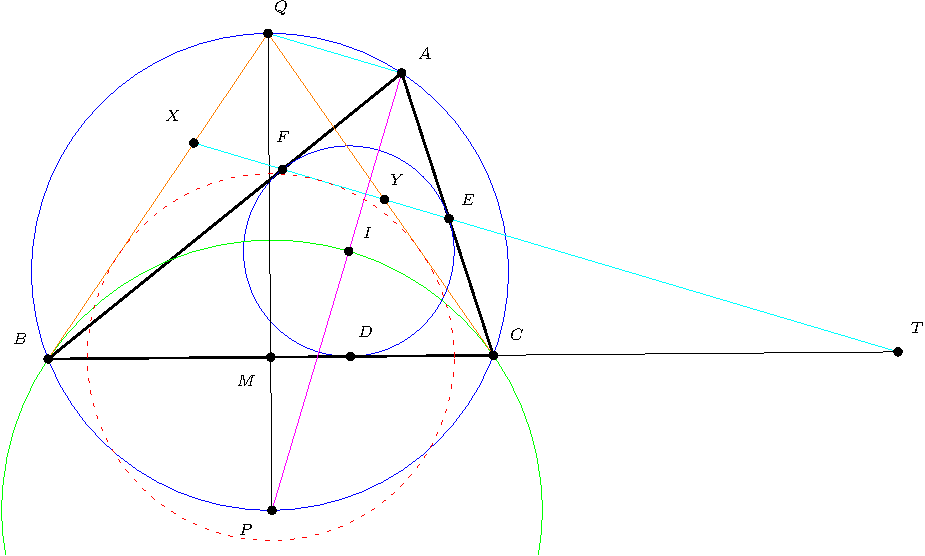
\includegraphics[width=0.9\textwidth]{hard_1_diagram-cropped.pdf}
    \end{flushright}
\end{figure}
\vfill
\newpage
\subsection{Solutions}
\subsubsection{Solution 1 (Fedir Yudin)}
We claim $M$ is the centre of the desired circle. To prove this, we will show the distances of $M$ to $\ell_B$, $\ell_C$ and $EF$ are equal.
\nl
Since $M$ is the midpoint of $BC$, we have
$$d(M, EF)=\frac{d(B, EF)+d(C, EF)}{2}.$$
Let $\alpha=\angle BAI=\angle IAC=\frac{1}{2}\angle BAC$. By considering the lines parallel to $AI$ going through $B$ and $C$, we can see
$$\frac{d(B, EF)+d(C, EF)}{2}=\frac{BF\cdot\cos\alpha+CE\cdot\cos\alpha}{2}=\frac{(BD+DC)\cos\alpha}{2}=MB\cos\alpha,$$
where the last equality holds since $BF=BD$ and $DC=EC$.
\nl
Since $QB$ is tangent to the circumcircle of $BIC$, we have
$$\angle BQM=90^\circ-\angle CBQ=90^\circ-(180^\circ-\angle BIC)=90^\circ-\angle CBI-\angle ICB=\alpha.$$
We conclude by noting that $MBQ$ and the triangle formed by $BM$, $\ell_B$ and the perpendicular from $M$ to $\ell_B$ are similar, which implies
$$MB\cos\alpha=d(M, \ell_B).$$
Due to symmetry, it is clear that $d(M, \ell_B)=d(M, \ell_C)$. Therefore, by combining the above relations, we obtain
$$d(M, EF)=d(M, \ell_B)=d(M, \ell_C).$$
Thus, $M$ is indeed the centre of the desired circle.
\nl
\subsubsection{Solution 2 (Navneel Singhal, Jakob Jurij Snoj)}
Let $\ell$ be the line tangent to the circumcircle of $BIC$ in $I$, which is clearly parallel to $EF$ and $AQ$. Since $\angle PQC=\angle PAC=\angle IAE$ and $\angle AEI=90^\circ=\angle QCP$ due to $PQ$ being the diameter of the circumcircle of $ABC$, the triangles $AEI$ and $QCP$ are similar.
\nl
Since $AEI$ and $QCP$ are similar triangles and $BC$ and $EF$ their altitudes, we can now compute:
$$\frac{d(Q, EF)}{d(Q, \ell)}=\frac{d(A, EF)}{d(A, \ell)}=\frac{QM}{QP}.$$
\nl
Observe the homothety centred in $Q$ taking $P$ to $M$. As it preserves tangency, it sends the circumcircle of $BIC$ to another circle $\omega$, tangent to $\ell_B$ and $\ell_C$, centred in $M$. Additionally, due to the above equality, it sends $\ell$ to $EF$. Since $\ell$ is tangent to the circumcircle of $BIC$, $EF$ is tangent to $\omega$. It follows that $\omega$ is the desired circle.
\subsubsection{Solution 3 (Massimiliano Foschi, Navneel Singhal)}
Note $B$, $C$, $E$ and $X$ are concyclic since $\angle BXE=180^\circ-\angle ACB$.
\nl
Observe that, since $AD$, $BE$ and $CF$ are concurrent, the harmonic property of complete quadrilaterals implies $T$ and $D$ are harmonic conjugates with respect to $A$ and $B$. In particular, we have $TD\cdot TM=TB\cdot TC$, since $TD$ and $TM$ are harmonic and arithmetic means, respectively, of $TB$ and $TC$.
\nl
By taking the power of point $T$ with respect to the circumcircle of $BCEX$, we now obtain
$$TE\cdot TX=TB\cdot TC=TM\cdot TD,$$
which implies $E$, $X$, $M$ and $D$ are concyclic.
\nl
We can now obtain
$$\angle MXE=\angle CDE=\frac{180^\circ-\angle ACB}{2}=\frac{\angle BXE}{2},$$
which implies $XM$ is the angle bisector of $\angle BXY$. Analogously, we obtain $YM$ is the angle bisector of $\angle XYC$. This implies $M$ is the centre of the $Q$-excircle of $QXY$, which concludes the proof.
\subsubsection{Solution 4 (Pitchayut Saengrungkongka)}
Since $AQ$ is parallel to $EF$, we have
$$\frac{FX}{QA}=\frac{BF}{BA}\qquad\text{and}\qquad \frac{EY}{QA}=\frac{CE}{CA}.$$
By Menelaus' Theorem for triangle $AEF$ and line $BC$, we have
$$\frac{AC}{CE}\cdot\frac{ET}{TF}\cdot\frac{FB}{BA}=1,$$
which, along with the above equalities, implies
$$\frac{TE}{TF}=\frac{EY}{FX}.$$
Let $M'$ be the excentre of the $Q$-excircle of $QXY$ (the desired circle). Since
$$\angle M'XY=\frac{\angle BXY}{2}=\frac{\angle BQA}{2}=\angle CDE=\angle DFE,$$
$XM'$ is parallel to $FD$. We conclude by noting the homothety centred in $T$ which takes $E$ to $Y$ evidently also takes $F$ to $X$ and $D$ to $M'$. It follows that $M'$ indeed lies on $BC$ as desired.
\subsubsection{Solution 5 (Pitchayut Saengrungkongka)}
Since $AQ$ is parallel to $EF$, we have
$$\angle XFB=\angle QAB=\angle QCB=\angle TBX,$$
therefore, $BXT$ and $FXB$ are similar triangles. Similarly, we can prove $\angle YEC=\angle TCY$, therefore $TCY$ and $YEC$ are similar triangles. It follows
$$TX=TB\cdot \frac{BX}{FB}\quad\text{and}\quad FX=FB\cdot\frac{XB}{BT},\quad\text{therefore}\quad\frac{TX}{FX}=\frac{TB^2}{BF^2}.$$
Similarly, we obtain $TY/EY=TC^2/CE^2$. We will now prove these two quantities are equal.
\nl
As in Solution 3, we prove $(B, C; D, T)=-1$. It follows that
$$\frac{TX}{FX}=\frac{TB^2}{BF^2}=\frac{TB^2}{BD^2}=\frac{TC^2}{CD^2}=\frac{TC^2}{CE^2}=\frac{TY}{EY}.$$
We conclude analogously to Solution 4 by defining $M'$ and observing the homothety from $T$ taking $X$ to $F$ and $Y$ to $E$ also takes $M'$ to $D$, therefore, $M'$ lies on $BC$ as desired.
\subsubsection{Solution 6 (Pitchayut Saengrungkongka)}
As in the other solutions, we prove $(B, C; D, T)=-1$. It follows that
$$MD\cdot MT=MB\cdot MC=MP\cdot MQ,$$
which implies $MDP$ and $MTQ$ are similar triangles (in particular, this shows $D$ is the orthocentre of $PQT$).
\nl
Let $I_A$ be the centre of the $A$-excircle of $ABC$. It is well known that the incircle and excircle tangency points on a triangle side are symmetric with respect to the side's midpoint. A homothety centred in $A$ sends $D$ to the point diametrically opposite the excircle tangency point on $BC$ on the $A$-excircle of $ABC$, which implies this point is collinear with $A$ and $D$. Together with the above, this implies $MI_A$ and $AD$ are parallel by observing a homothety with ratio $1/2$ centred in the tangency point of the $A$-excircle and $BC$.\nl
The triangles $DIA$ and $MPI_A$ therefore have pairwise parallel sides and are thus similar. In particular, let $G$ be the intersection of $BC$ and $AI$. The point $G$ is the centre of the homothety taking $DIA$ to $MP_IA$, which implies $$\frac{DG}{GM}=\frac{AG}{GI_A}.$$
Recall once again $PMD$ and $TMQ$ are similar triangles, as well as $\angle HTM=\angle APH$. This implies $DG/GM=QH/HM$ and therefore,
$$\frac{QH}{HM}=\frac{AG}{GI_A}.$$
We conclude by noting the triangles $ABC$ and $QYX$ are similar. Indeed, $$\angle ACB=180^\circ-\angle BQA=180^\circ-\angle BXY=\angle YXQ\quad\text{and}\quad  \angle XQY=\angle BAC.$$
Since $AI$ and $QM$ are respective angle bisectors in these triangles, the equality $QH/HM=AG/GI_A$ implies that, since $I_A$ is the excenter opposite $A$ of $ABC$, $M$ is the excenter opposite $Q$ of $QXY$. The $Q$-excircle of $QXY$ is precisely the desired circle, which concludes the proof.

\subsubsection{Solution 7 (Pitchayut Saengrungkongka)}

We use barycentric coordinates with respect to $\triangle ABC$, i.e. point $(x,y,z)$ where $x+y+z=1$ will refer to $x\vec{A}+y\vec{B}+z\vec{C}$. We also use the notation $(kx:ky:kz)$ to denote point $(x,y,z)$ for any $k\in\mathbb{R}$.
\nl
Set $a=BC, b=CA, c=AB$. It's easy to see that $I=(a:b:c)$, $E=(s-c:0:s-a)$ and $F=(s-b:s-a:0)$. Now we proceed to compute $Q$. Since $Q$ lies on the $A$-external bisector, it follows that $Q=(t:-b:c)$ for some $t\in\mathbb{R}$. As in Solution 2, we get that $Q$ lies on the circumcircle of $ABC$. Thus by plugging in this into the circumcircle equation, we get 
$$a^2(-b)(c) + b^2(t)(c) + c^2(-b)(t)=0 \implies t = \frac{a^2}{c-b}$$
Thus $Q$ has coordinate $(-a^2: b(b-c):c(c-b))$. Now to compute $X$, one could intersect $BS$ with $EF$ directly. But this requires factorization of asymmetric expression, so we will present a simpler approach: let $X'$ be the point on $BS$ such that $MX'\parallel DF$ and we aim to show that $X'\in EF$.
\nl
To compute $X'$, note that since $X'\in BS$, there exists $t\in\mathbb{R}$ such that $X' = (-a^2:t:c(c-b))$. Clearly, $M$ has the coordinate $(0:1:1)$ while $\infty_{DF}$ has the coordinate $(a:c-a:-c)$ (as it's also the point at infinity along the $B$-external bisector). By Shoelace formula, we get that
$$0 = \det\begin{bmatrix}
    0 & 1 & 1 \\
    a & c-a & -c \\
    -a^2 & t & c(c-b)
\end{bmatrix}  = a\det\begin{bmatrix}
    0 & 1 & 1 \\
    1 & c-a & -c \\
    -a & t & c(c-b)
\end{bmatrix}
$$ 
Expanding via minors (on the first row), we find that
$$\det\begin{bmatrix}
    1 & -c \\
    -a & c(c-b)
\end{bmatrix} = \det\begin{bmatrix}
    1 & c-a \\
    -a & t
\end{bmatrix} \implies t+a(c-a) = c(c-b)-ac$$
Thus $t=a^2+c^2-bc-2ac$. Therefore $X' = (-a^2 : a^2+c^2-bc-2ac : c(c-b))$. To show that this point lies on $EF$, we need to show that
$$\det\begin{bmatrix}
    -a^2 & a^2+c^2-bc-2ac & c^2-bc \\
    s-c & 0 & s-a \\
    s-b & s-a & 0
\end{bmatrix} = 0$$
Expanding the determinant, we have to show that
$$(a^2+c^2-bc-2ac)(s-a)(s-b)+c(c-b)(s-c)(s-a)=-a^2(s-a)^2.$$
Dividing by $s-a$, and multiplying both sides by $2$, it suffices to show that
$$(a^2+c^2-bc-2ac)(a+c-b) + c(c-b)(a+b-c) + a^2(b+c-a)=0.$$
The first term is
\begin{align*}
    (a^2+c^2-bc-2ac)(a+c-b) &= (a^3+ac^2-abc-2a^2c)+(a^2c+c^3-bc^2-2ac^2) \\
    &\qquad - (a^2b+c^2b-b^2c-2abc) \\
    &= a^3-ac^2+abc-a^2c+c^3-2bc^2-a^2b+b^2c
\end{align*}
while the last two terms combined is
\begin{align*}
    &c(ac+bc-c^2-ab-b^2+bc) + a^2(b+c-a) \\ =\ &  ac^2+2bc^2-c^3-abc-b^2c+a^2b+a^2c-a^3
\end{align*}
It's clear that all add up to $0$ so we get that $X'\in EF$ so $X'=X$. This completes the problem as we have $MX\parallel DF$ thus $\angle MXE = \angle DFE = 90^{\circ}-\tfrac C2$ and $\angle MXY = \angle AQX = \angle C$ hence $MX$ bisects $\angle BXE$.
\subsubsection{Solution 8a (Navneel Singhal)}
We first prove another stronger property of the configuration: the circumcircle of $QXY$ is tangent to the circumcircle of $BIC$.
\nl
Note that, by the Right Angles on Intouch Chord Lemma, we need to show the following:
\nl
Let $ABC$ be a triangle, and let $A'B'C'$ be its orthic triangle, and $H$ its orthocenter. Let the tangents to the circumcircle of $BHC$ at $B$ and $C$ and the line $B'C'$ form a triangle $GUV$, with $G$ being on both tangents, and $V$ being on that from $C$. Then the circumcircle of $GUV$ is tangent to the circumcircle of $BHC$.
\nl
This can be done using Casey's theorem, however we follow a more synthetic approach.\nl
We claim that the point of tangency is $K$, the $A$-Humpty point. 
Let $U'$ be the point where $B'C'$ meets the circumcircle of $BFKM$ (where $M$ is the midpoint of $BC$). Then we have $\angle U'BK = \angle U'C'K = \angle B'C'K = \angle B'AK = \angle KCB = \angle UBK$, so $U = U'$.
\nl
Also $\angle UKB = \angle UKC' + \angle C'KB = \angle UBC' + \angle C'MB = \angle B - \angle A + 2\angle C'CB = \angle C = \angle B'CK + \angle KCB = \angle UVK + \angle KCB$, so the circumcircle of $UKV$ is tangent to the circumcircle of $BKC$, which is also the circumcircle of $BHC$.
\nl
Now by Miquel's theorem on triangle $GBC$ and points $U, V, M$, we have $K$ on the circumcircle of $GUV$ too, so we are done.
\nl
We now conclude by noting that $\angle BUM = \angle BC'M = \angle MBC' = \angle MUE$ (which does not need the full power of the result), or by simply using the properties of the mixtilinear excircle (the midpoint of the touchchord of the mixtilinear excircle is the corresponding excentre).
\subsubsection{Solution 8b (Pitchayut Saengrungkongka)}
Let $E_1$ and $F_1$ be the intersections of $BI$ and $CI$, respectively, with $EF$. Note that, by the Right Angles on Intouch Chord Lemma, we have $MB=MC=ME_1=MF_1$.
\nl
It follows that
$$\angle CME_1=180^\circ-\angle E_1MB=2\angle MBI=\angle MBA=\angle CYE,$$
therefore, the points $C$, $M$, $Y$ and $E_1$ are concyclic. We can now conclude by noting
$$\angle XYM=\angle E_1CM=\angle ME_1C=\angle MYC,$$
from which it follows that $YM$ is the angle bisector of $XYC$. By showing analogously that $XM$ is the angle bisector of $BXY$ or remarking $QM$ is the angle bisector of $BQC$, it follows that $M$ is indeed the desired excentre.
\subsubsection{Solution 8c (Navneel Singhal)}
We define $E_1$ and $F_1$ as in Solution 8b. Since $AQ\parallel EF$, it follows by Reim's Theorem that $B$, $F$, $Y$ and $C$ are concyclic. By the extended Right Angles on Intouch Chord Lemma, $E_1$ lies on the line connecting the midpoints of $BC$ and $CA$. Since this line is parallel to $BF$, it follows by Reim's Theorem that $M$, $C$, $E_1$ and $Y$ are concyclic. We now finish as in Solution 8b.
\subsubsection{Solution 9 (Pitchayut Saengrungkongka)}
Let $H$ be the orthocenter of $BIC$, $K$ be the midpoint of $BH$ and $B_1, C_1$ be the feet of perpendiculars from $C$ to $HB$ and $B$ to $HC$. From the Right Angles on Intouch Chord Lemma, $B_1$,  $C_1$, $E$, $F$ are colinear.
\nl
As $DI\perp BC$, the points $K$, $M$, $D$, $B_1$ and $C_1$ all lie on the nine-point circle of $BCH$. We now apply Pascal's theorem on $KMDB_1C_1K$ to get that $KM \cap EF$, $MD \cap C_1K$ and $KK \cap DB_1$ are collinear. Note that, since $D$, $I$, $B_1$ and $C$ are concyclic,
$$\angle CDB_1 = \angle CIB_1= 180^\circ-\angle BIC=\angle CBI+\angle ICB=90^\circ-\angle BAI90^\circ-\angle BQP=\angle CBQ,$$ so $BQ \parallel DB_1$. Now, since $KD=KB_1$ due to Thales' Theorem, $K$ is the midpoint of arc $DC_1B_1$ in the nine-point circle of $BIC$. It follows the tangent at $K$ to it is parallel to $DB_1$. From the result we obtained by using Pascal's Theorem, it now follows that $KM\cap EF=X$.
\nl
Since
$$\angle C_1B_1I=\angle C_1HI=\angle C_1HD=\angle C_1CD=\angle ICD=\angle IB_1D,$$ $HC$ is one of the angle bisectors of $EF$ and $DB_1$. Since $DB_1\parallel BQ$ and $CH\parallel MK$ and since $X=KM\cap EF$ lies on $BQ$, it follows that $XM$ is also an angle bisector of $\angle BXY$. It follows that $M$ is the desired excentre, which concludes the proof.
\subsubsection{Solution 10 (Amirhosein Rajabi)}
Without loss of generality, we can assume $\angle B \ge \angle C$. One can see that $AQ$ is parallel to $EF$ and we have that since $\angle AEX = \angle QBC$, $XECB$ is a cyclic quadrilateral. Let the bisectors of the angles between $EF$ and $BQ$ intersect $BC$ at $L$ and $N$ (with $L$ between $B$ and $T$). Therefore, $(T, B; L, N) = -1$. Also it is known that $(T, D; B, C) = -1$. Now we use the similarity of triangles $TXB$ and $TCE$ (because of the cyclic quadrilateral $XECB$) along with these harmonic ratios to obtain
\begin{align*}
    \frac{BT}{BD} = \frac{TC}{CD}
    = \frac{TC}{CE}
    = \frac{TX}{XB}
    = \frac{TL}{LB}
    = \frac{NT}{BN}
    = \frac{NB + BT}{DN + BD}
    = \frac{NB}{DN}
\end{align*}
This means $\frac{NT}{BN} = \frac{NB}{DN}$, which gives us $NB^2 = ND \cdot NT$. So the reflection of $B$ over $N$ is the point $C'$ such that $(B, C'; D, T) = -1$, and since $(B, C; D, T) = -1$, we have $C = C'$, so $N$ is the midpoint of $BC$, and we are done.
\subsection{Preliminary notes on grading this problem}
\begin{enumerate}
    \item Any complete solutions should be awarded a full 7 points, regardless of whether they fit in the marking scheme or not.
    \item Partial credits across different approaches are \textbf{not} additive. If a student has a partial solution that can be graded via different marking schemes, the one which leads to the highest score should be followed.
    \item Any partial solutions that can lead to solutions, but which are not outlined in one of the following cases, should be graded equivalently.
    \item If you are not sure if a partial solution can lead to a solution or not, you could discuss this with other graders and if that turns out to be inconclusive, the members of the problem selection committee.
    \item Non-trivial but minor errors in a complete solution usually lead to a deduction of 1 point.
    \item No points are deducted if a contestant fails to handle possible configuration issues (such as not using directed angles).
    \item No points are deducted for quoting well known results without proof (including, but not limited to, Right Angles on Intouch Chord Lemma, Incentre-Excentre Lemma and the harmonic property of complete quadrilaterals).
    \item \textbf{Caveat:} Points for computational approaches should only be awarded if the results are interpreted synthetically.
\end{enumerate}

\subsection{Marking scheme}
In every sub-enumeration, the mentioned partials are given, if the mentioned part of the solution has not been completed. For example, if in the first solution, someone has not expressed $d(M, EF)$ as described, but has proven $d(M, EF)=(d(B, EF)+d(C, EF))/2$, the contestant would get 1 point for that part of the solution. The points within the sub-enumerations are \textbf{not} additive, unless mentioned explicitly.

\subsubsection{Solution 1 (Fedir Yudin)}
\begin{enumerate}
        \marking{1}{Expressing $d(M, l_B)$ or $d(M, l_C)$ only in terms of $MB$, $MC$ or $BC$ and $\alpha$ (such as $MB\cos\alpha$)}
        \marking{5}{Expressing $d(M, EF)$ only in terms of $MB$, $MC$ or $BC$ and $\alpha$ (such as $MB\cos\alpha$)}
        \begin{enumerate}
                \marking{1}{Proving $d(M, EF)=(d(B, EF)+d(C, EF))/2$}
                \marking{3}{Proving $d(M, EF)=((BF+CE)\cos\alpha)/2$}
        \end{enumerate}
        \marking{1}{Argumenting $d(M, \ell_B)=d(M, \ell_C)=d(M, EF)$, which implies $M$ is the desired centre (this point can only be given if 1. and 2. are both proven)}
\end{enumerate}
\subsubsection{Solution 2 (Navneel Singhal, Jakob Jurij Snoj)}
\begin{enumerate}
        \marking{1}{Proving $AQ\parallel EF$ \textbf{and} proving $Q$ lies on the circumcircle of $ABC$}
        \marking{2}{Reducing the problem to proving $d(Q, EF)/d(Q, \ell)=QM/QP$}
        \begin{enumerate}
                \marking{1}{Only mentioning a homothety centred in $Q$ which sends the circumcircle of $BIC$ to the desired circle without making the above reduction}
        \end{enumerate}
        \marking{4}{Proving $d(Q, EF)/d(Q, \ell)=QM/QP$}

        The following partial points are \textbf{additive}:
        \begin{enumerate}
                \marking{1}{Proving $d(Q, EF)/d(Q, \ell)=d(A, EF)/d(A, \ell)$}
                \marking{1}{Proving $AEI$ and $QCP$ are similar triangles}
        \end{enumerate}
\end{enumerate}
\subsubsection{Solution 3 (Massimiliano Foschi, Navneel Singhal)}
\begin{enumerate}
        \marking{2}{Proving $B$, $C$, $E$, $X$ are concyclic or proving $B$, $C$, $F$, $Y$ are concyclic}
        \begin{enumerate}
                \marking{1}{Proving $AQ\parallel EF$ \textbf{and} proving $Q$ lies on the circumcircle of $ABC$}
        \end{enumerate}
        \marking{4}{Proving $M$, $D$, $E$, $X$ are concyclic or proving $M$, $D$, $F$, $Y$ are concyclic}
        \begin{enumerate}
                \marking{1}{Proving $(B, C; D, T)=1$}
        \end{enumerate}
        \marking{1}{Reducing the problem to one of the concyclicities in 2.}
\end{enumerate}

\subsubsection{Solutions 4 and 5 (Pitchayut Saengrungkongka)}
\begin{enumerate}
        \marking{2}{Reducing the problem to showing the homothety sending $EY$ to $FX$ is centred at $T$ (or an equivalent statement)}
        \begin{enumerate}
                \marking{1}{Only defining the desired excentre $M'$ \textbf{and} proving $XM'\parallel FD$ or $YM'\parallel ED$, but not explicitly reducing the problem}
        \end{enumerate}
        \marking{5}{Proving the homothety sending $EY$ to $FX$ is centred at $T$ (or an equivalent statement)}
        \begin{enumerate}
                \marking{2}{Proving $FX/QA=BF/BA$ \textbf{or} $EY/QA=CE/CA$ \textbf{or} $BXT$ and $FXB$ are similar triangles \textbf{or} $TCY$ and $YEC$ are similar triangles}
                \marking{2}{Only using the Menelaus' theorem for triangle $AEF$ and line $BC$ or proving an equivalent statement which would, together with (a), imply 2.}
                \marking{1}{Only showing $(B, C; D, T)=-1$}
                \marking{3}{Proving $TX/FX=TB^2/BF^2$ or $TY/EY=TC^2/CE^2$}
                \marking{4}{Proving length relations that would, only with algebraic manipulation, be sufficient to establish 2., but failing to complete the proof}
                \marking{1}{Proving $AQ\parallel EF$ (this point is \textbf{additive only with (b) and (c)})}
        \end{enumerate}
\end{enumerate}
\subsubsection{Solution 6 (Pitchayut Saengrungkongka)}
\begin{enumerate}
        \marking{2}{Proving $M$, $Q$, $T$, $D$ form an orthocentric system}
        \begin{enumerate}
                \marking{1}{Only showing $(B, C; D, T)=-1$}
        \end{enumerate}
        \marking{2}{Proving $DG/GM=AG/GI_A$}
        \begin{enumerate}
                \marking{1}{Proving $MI_A\parallel AD$}
        \end{enumerate}
        \marking{3}{Reducing the problem to $DG/GM=AG/GI_A$}
        \begin{enumerate}
                \marking{2}{Only reducing the problem to $QH/HM=AG/GI_A$, regardless of whether 1. was completed}
                \marking{1}{Only proving $ABC$ and $QYX$ are similar or an equivalent statement}
                \marking{1}{Only proving $DG/GM=QH/HM$}
                \marking{2}{Proving (b) and (c), but failing to complete the proof}
        \end{enumerate}
\end{enumerate}
\subsubsection{Solutions 8 and 9 (Navneel Singhal, Pitchayut Saengrungkongka)}
\begin{enumerate}
        \marking{2}{Defining $E_1$ and $F_1$ such as in Solution 8b or equivalent \textbf{and} using the Right Angles on Intouch Chord Lemma to prove their properties, thus transforming the problem as in one of these solutions (for example, defining $E_1$ and $F_1$ in Solution 8b and proving $MB=MC=ME_1=MF_1$ or $BE_1\perp E_1C$ in the same notation, such as in Solution 9)}
        \marking{5}{Solving the transformed problem}
        \begin{enumerate}
                \marking{1}{Only proving $ABC$ and $QYX$ are similar, $B$, $C$, $Y$, $F$ or $B$, $C$, $E$, $X$ are concyclic or an equivalent statement}
                \marking{3}{Proving $M$, $C$, $E_1$, $Y$ or $M$, $B$, $F_1$, $X$ (in notation of 8b) are concyclic}
                \marking{2}{Using Pascal's Theorem such as in Solution 9 in a way that allows the contestant to finish in an analogous manner}
                \marking{3}{Proving $M$, $K$ and $X$ are collinear}
        \end{enumerate}
\end{enumerate}
\subsubsection{Solution 10 (Amirhosein Rajabi)}
\begin{enumerate}
        \marking{1}{Proving $X$, $E$, $C$ and $B$ are concyclic or proving $Y$, $F$, $C$ and $B$ are concyclic}
        \marking{5}{Obtaining $NT/BN=NB/DN$ or equivalent, where $N$ is defined as the intersection of the internal bisector of $\angle BXY$ or $\angle XYC$ and line $BC$}
        \begin{enumerate}
                \marking{2}{Observing $L$ and $N$ and establishing $(T, B; L, N)=-1$ \textbf{and} $(T, D; B, C)=-1$}
                \marking{1}{Proving only one of the two harmonic ratios}
        \end{enumerate}
        \marking{1}{Reducing the problem to $NT/BN=NB/DN$, where $N$ is defined as in 2.} 
\end{enumerate}
 %not final - need to add diagram and markscheme for solution 10
\pagebreak
\section{Problem 2}
\subsection{Problem}
Geoff has an infinite stock of sweets, which come in $n$ flavours. He arbitrarily distributes some of the sweets amongst $n$ children (a child can get sweets of any subset of all flavours, including the empty set). Call a distribution of sweets $k$\emph{-nice} if every group of $k$ children together has sweets in at least $k$ flavours. Find all subsets $S$ of $\{1,2,\dots,n\}$ such that if a distribution of sweets is $s$-nice for all $s\in S$, then it is $s$-nice for all $s\in \{1,2,\dots,n\}$.\nl
\textit{Proposed by Kyle Hess, USA}

\subsection{Solutions}
We claim that $S = \{1, 2, \dots, n\}$ is the only $S$ that satisfies the problem conditions. It is clear that it does. Now we show that this is the only one.\nl
Consider the obvious translation to the language of bipartite graphs, where one part represents children and the second one represents flavours, and two vertices are connected if and only if the respective child has a sweet of the respective flavour. We show that for each $r \in \{1, 2, \dots, n\}$, there exists a bipartite graph (with two $n$-sized partitions) that is not $r$-nice but is $s$-nice for all $\in\{1,2,\dots,n\}\setminus\{r\}$. Then for every $S\neq \{1,2,\dots,n\}$ our construction for some $r\in \{1,2,\dots,n\}\setminus S$ proves that $S$ doesn't satisfy problem conditions.

\subsubsection{Solution 1 (David Rusch)}
We take the bipartite graph $\{1,\dots, r\} \times \{1,\dots,r-1\} \cup \{r+1,\dots,n\} \times \{1,\dots,n\}$. Note that the sets are defined to be empty if they don't make sense ($r=1$ or $r=n$). Now, $r$ doesn't work because of $\{1,2,\dots,r\}$, but every other $s$ works obviously. If $s<r$, there are at least $r-1$ neighbors no matter what and if $s>r$, there are $n$ neighbours. 

\subsubsection{Solution 2 (Navneel Singhal)}
We construct such bipartite graphs by induction. The case for $\{1, 2\}$ is easy to see.\nl
Now suppose we have such examples for $n$. We wish to exhibit such examples for $n+1$. We break into two cases: $r \ne n+1$ and $r = n+1$.\nl
Firstly suppose $r \ne n+1$. For this case, join $n+1$ on the left to all vertices on the right, then utilise the construction for the same subset without $n+1$ using the induction hypothesis, for the vertices $1$ to $n$. It's easy to see that this is not $f$ expanding only for $f = r$.\nl
Now we do the case $r = n+1$. For this case, we do this construction: $k$ on the left is adjacent to all the vertices $i$ on the right such that $i \le k$, and $n+1$ is joined to $\{1, 2, \dots, n\}$. For any subset of the vertices on the left of size $g \le n$, there is at least one vertex whose index is at least $g$, or there is $n+1$ in it, so the size of $R(S)$ is $\ge g$, and thus $|R(S)| \ge |S|$. However since the set of neighbours of all the vertices on the left is of size $n$,
the graph this construction leads to is not $n+1$-nice.\nl
This implies, by induction, that for every $n$, there for each $r \in \{1, 2, \dots, n\}$, there exists a bipartite graph (with 2 $n$-sized partitions) that is not $r$-nice but is $s$-nice for all $s \ne r$, $r, s \in \{1, 2, \dots, n\}$.

\subsection{Marking scheme}
\begin{enumerate}
        \marking{0}{Only mentioning the correct answer}
        \marking{1}{Showing that it suffices to prove that for every $r\in\{1,2,\dots,n\}$ there is a distribution that is not $r$-nice but is $s$-nice for all $s\in\{1,2,\dots,n\}\setminus\{r\}$ to solve the problem}
        \marking{6}{For every $r\in\{1,2,\dots,n\}$, constructing a distribution that is that is not $r$-nice but is $s$-nice for all $s\in\{1,2,\dots,n\}\setminus\{r\}$}
        \begin{enumerate}
                \marking{1}{constructing such a distribution for some particular value of $r$}
        \end{enumerate}
        \marking{-0}{Claiming that a construction works without proving it (when it is indeed easy to see)}
\end{enumerate}



\pagebreak
\section{Problem 3}
\subsection{Problem}
We call a set of integers \textit{special} if it has 4 elements and can be partitioned into 2 disjoint subsets $\{a,b\}$ and $\{c,d\}$ such that $ab-cd=1$. For every positive integer $n$, prove that the set $\{1,2, \ldots , 4n\}$ cannot be partitioned into $n$ disjoint special sets.\nl
\textit{Proposed by Mohsen Jamali, Iran}

\subsection{Solutions}
We assume, for the sake of contradiction, that we can partition the set $\{1,2,\hdots , 4n\}$ into $n$ disjoint special sets $S_1, S_2,\hdots , S_n$. Every special set contains at most 2 even integers since it can be partitioned so that $ab-cd=1$. But there're exactly $2n$ even and $2n$ odd numbers, thus each $S_i$ must contain exactly 2 even and 2 odd integers, and the numbers with same parity are paired to each other. Let's call $S_i=\{a_i, b_i, c_i, d_i\}$ with $a_i,b_i$ even, $c_i,d_i$ odd, and $a_ib_i-c_id_i=\pm 1$.
\nl Note that  $\displaystyle{\bigcup_{i=1}^n\ \{a_i,b_i\}=\{2,4,\hdots , 4n\}}$ and  $\displaystyle{\bigcup_{i=1}^n\ \{c_i,d_i\}=\{1,3,\hdots , 4n-1\}}$.
\nl Next, we provide two different solutions that lead to the contradiction of our assumption.

\subsubsection{Solution 1 (Morteza Saghafian)}
Observe that $a_ib_i=c_id_i\pm 1\leq c_id_i+1<(c_i+1)(d_i+1)$. Multiplying these equations for $i=1,2,\hdots , n$ yields
\begin{align*}
    2\cdot4\cdot \hdots \cdot 4n &= \prod_{i=1}^n\ a_ib_i \\
    &< \prod_{i=1}^n\ (c_i+1)(d_i+1) \\
    &= 2\cdot 4 \cdot \hdots \cdot 4n,
\end{align*} which is impossible. This contradiction completes the proof.

\subsubsection{Solution 2 (Natanon Therdpraisan)}
Observe that $a_ib_i=c_id_i\pm 1\leq c_id_i+1$. Multiplying all equations gives $$2\cdot 4\cdot \hdots \cdot 4n=\prod_{i=1}^n\ a_ib_i\leq \prod_{i=1}^n\ (c_id_i+1).$$
Consider any positive real numbers $x_1<x_2<x_3<x_4$. By rearrangement inequality, we know that $$(x_{j_1}x_{j_2}+1)(x_{j_3}x_{j_4}+1)\leq (x_1x_2+1)(x_3x_4+1)$$ for any permutation $(j_1,j_2,j_3,j_4)$ of $(1,2,3,4)$.
\nl Hence, 
\begin{align*}
    \prod_{i=1}^n\ (c_id_i+1)&\leq \prod_{t=1}^n\ ((4t-3)(4t-1)+1) \\
    &< \prod_{t=1}^n\ (4t-2)(4t) \\
    &= 2\cdot 4 \cdot \hdots \cdot 4n,
\end{align*} which is clearly a contradiction and the proof completes.

\subsubsection{Remark}
The above solutions all approach by putting $\pm 1$ on the odd side, multiplying all equations together, and then comparing the product of all even pairs and the product of all odd pairs (with $\pm1$ added to each pair). However, the solution can still be done similarly if $\pm 1$ is put on the even side, i.e. 
\nl for solution 1, we use $c_id_i=a_ib_i\pm 1\geq a_ib_i-1>(a_i-1)(b_i-1)$ ;
\nl for solution 2, rearrangement inequality implies $(x_{j_1}x_{j_2}-1)(x_{j_3}x_{j_4}-1)\geq (x_1x_2-1)(x_3x_4-1)$, and thus $$\prod_{i=1}^n\ (a_ib_i\pm 1)\geq \prod_{t=1}^n\ ((4t-2)(4t)-1)>\prod_{t=1}^n\ (4t-3)(4t-1).$$
\nl Therefore, the marking scheme below should also apply equivalently if such approach happens.



\subsection{Marking scheme}
To our knowledge, we don’t know any substantially different approach to this problem. If such approach happens, it should be judged as equivalently as possible. The marking scheme is divided into two additive parts. However, partial credits within each part are \textbf{not} additive.

\begin{enumerate}
        \marking{0}{Examples of non-rewarding observations:}
        \begin{enumerate}
            \item Casework specific value(s) of $n$ that does not give insight to general case
            \item Show that each special set has exactly one way of partition, e.g. if $ab-cd=1$ then $|ac-bd|,|ad-bc|\neq 1$
            \item Show that $gcd\ (a,c)=1$ etc.
        \end{enumerate}
        \marking{2}{Showing that each special subset contains exactly 2 even and 2 odd integers, and numbers with same parity are paired to each other}
        \begin{enumerate}
                \marking{1}{Prove that each special subset contains at most 2 even numbers}
                \marking{1}{Prove that each special subset contains at least 2 odd numbers}
                \marking{1}{Prove that each special subset contains exactly 2 even and 2 odd numbers}
        \end{enumerate}
        \marking{5}{Completing the solution}
        \begin{enumerate}
                \marking{2}{Attempt to contradict the assumption by comparing the sizes of the product of all even pairs and that of all odd pairs, e.g. multiplying all $n$ equations, or claiming that the product of all even pairs is still strictly more than the product of all odd pairs after plus 1 to each pair}
                \marking{2}{Show or mention (since it's easy to prove) that $xy\pm 1<(x+1)(y+1)$ for any $x,y>0$}
                \marking{2}{Prove that the product of all odd pairs with 1 added to each pair maximizes when the numbers with more values are paired to each other}
                \marking{1}{Claim (c), without justification}
                \marking{0}{Show or mention that $xy\pm 1\leq xy+1$ for any real number $x,y$}
        \end{enumerate}
\end{enumerate}
The correct solutions should be judged as 7 even if they're different from the above solutions. However, the following deductions could be applied:
\begin{enumerate}\setcounter{enumi}{3}
        \marking{-1}{The contestant has proven that each special subset contains 2 even and 2 odd integers, but use the fact that in each special subset each number must be paired only with one of same parity without mentioning}
        \marking{-1}{The contestant has any other non-trivial minor error}
\end{enumerate}



\pagebreak
\section{Problem 4}
\subsection{Problem}
Prove that for all sufficiently large integers $n$, there exist $n$ numbers $a_1,a_2,\ldots,a_n$ satisfying the following three conditions:
\begin{enumerate}
    \item Each number $a_i$ is equal to either $-1$, $0$ or $1$.
    \item At least $2n/5$ of the numbers  $a_1,a_2,\ldots, a_n$ are non-zero.
    \item $a_1/1+a_2/2+\ldots+a_n/n=0$.
\end{enumerate}
\textit{Proposed by Navneel Singhal, India, Kyle Hess, USA, and Vincent Jugé, France}

\subsection{Solutions}

\subsubsection{Solution 1 (Vincent Jugé)}

Let us say that a set $S \subseteq \{1,2,\ldots,n\}$ is $\emph{nice}$ if there exists a function $f : S \mapsto \{-1,1\}$ such that $\sum_{k \in S} f(k) / k = 0$; we say that $f$ is a $\emph{witness}$ for $S$.\nl
Thus, we prove below that, if $n$ is large enough, there exists a nice set of size at least $2n/5$. Note a disjoint union of two nice sets is nice. Hence, the first goal would be to identify many disjoint nice sets.
Aiming towards this goal, and due to the identity
\[1 - 1/2 - 1/3 - 1/6 = 0,\]we first see that each set $S_k = \{k,2k,3k,6k\}$, where $k \leq n/6$, is a nice set. However, we wish to have disjoint sets only, and therefore we will not consider all these sets at once.
\nl
Instead, let us check whether some integer $m$ can belong to two such sets $S_k$ and $S_\ell$, with $n/12 < k < \ell \leq n/6$.
Since\[n/12 < k < \ell \leq n/6 < 2k < \min\{3k,2\ell\} \leq \max\{3k,2\ell\} < 3\ell \leq n/2 < 6 k < 6 \ell,\]it follows that $m = 3 k = 2 \ell$.
\nl
This further implies that $k$ is even, with $n/2 < k = 2 \ell / 3 \leq n/9$, and that $\ell$ is divisible by $3$, with $n/8 < 3 k / 2 = \ell < n/6$.
\nl
Consequently, we can partition the set $\{k \in \mathbb{N} \colon n/12 < k \leq n/6\}$ into three subsets
\begin{align*}
    A & = \{k \in \mathbb{N} \colon n / 12 < k \leq n/9 \text{ and }
    k \equiv 0 \hspace{-2mm}\pmod{2}\} \text{,} \\
    B & = \{k \in \mathbb{N} \colon n / 8 < k \leq n/6 \text{ and }
    k \equiv 0 \hspace{-2mm}\pmod{3}\} =
    \{3 k / 2 \colon k \in A\}  \text{ and} \\
    C & = \{k \in \mathbb{N} \colon n / 12 < k \leq n/6\} \setminus (A \cup B) \text{,}
\end{align*}
such that both families $(S_k)_{k \in A \cup C}$ and $(S_k)_{k \in B \cup C}$ are families of pairwise disjoint nice sets. However, we cannot use simultaneously sets $S_k$ and $S_\ell$ when $k \in A$ and $\ell \in B$.
\nl
Hence, we modify these sets as follows. Given some integer $k \in A$, let $\ell = 3k / 2 \in B$. Due to the identity
\begin{align*}
    0 & = (1-1/2-1/3-1/6)/2 - (1-1/2-1/3-1/6)/3 - (1/6 - 2/12) \\
    & = 1/2 - 1/3 - 1/4 - 1/6 + 1/9 + 1/12 + 1/18,
\end{align*}and although the intersection $S_k \cap S_\ell$ is non-empty, the set $S_k \cup S_\ell$ is still nice. Consequently, the sets $(S_k)_{k \in C} \cup (S_k \cup S_{3k/2})_{k \in A}$ form a family of pairwise disjoint nice sets. In particular, their union $\mathcal{S} = \bigcup_{n/12 < k \leq n/6} S_k$
is also nice, and its cardinality is $|\mathcal{S}| = 7 |A| + 4 |C| = 23n/ 72 - \mathcal{O}(1)$.
\nl
Finally, let $\mathcal{T}$ be a maximal nice set (for the inclusion) containing $\mathcal{S}$. Assume that some integer $k \leq n/12$ does $\emph{not}$ belong to $\mathcal{T}$. Let $\ell$ be the largest such integer, and let $f : \mathcal{T} \mapsto \{-1,1\}$ be a witness for $\mathcal{T}$. By maximality of $\ell$, we know that $2 \ell \in \mathcal{T}$. Then, let $\mathcal{T}' = \mathcal{T} \cup \{\ell\}$, and let $f' : \mathcal{T}' \mapsto \{-1,1\}$ be defined by $f'(\ell) = f(2\ell)$, $f'(2\ell) = -f(2\ell)$, and $f'(k) = f(k)$ otherwise. One checks easily that $f'$ is a witness for $\mathcal{T}'$, contradicting the maximality of $\mathcal{T}$.
\nl
We conclude that each integer $k \leq n/12$ also belongs to $\mathcal{T}$, and thus that $\mathcal{T}$ is a nice set of size $|\mathcal{T}| \geq |\mathcal{S}| + n / 12 + \mathcal{O}(1) = 29n/ 72 - \mathcal{O}(1)$. Since $29 / 72 > 2/5$, this completes the proof.

\subsubsection{Solution 2 (Navneel Singhal)}
We give an explicit construction of a nice tuple with $\frac 25$ replaced by $\frac13 - \varepsilon$, showing that the number of non-zero elements in such an $n-$tuple can be made $\frac{n}{3} - \mathcal{O}(\log^2 n)$.
Let $r = \left\lfloor \frac{N}{6}\right\rfloor$. Let $v_p(n)$ be the highest $e$ such that $p^e | n$ for a prime $p$. Let
$$
a_k = 
\begin{cases}
    1 & \text{if } v_2(k) \text{ and } v_3(k) \text{ are both even with } k \le r\\
    -1 & \text{if } v_2(k) \text{ is odd and } v_3(k) \text{ is even with } k \le 2r\\
    -1 & \text{if } v_2(k) \text{ is even and } v_3(k) \text{ is odd with } k \le 3r\\
    -1 & \text{if } v_2(k) \text{ and } v_3(k) \text{ are both odd with } k \le 6r\\
    0 & \text{otherwise}
\end{cases}
$$
Firstly we show that this construction works.
Consider the identity $1 - \frac12 - \frac13 - \frac16 = 0$. Consider integers $m$ not exceeding $r$, of the form $2^{2x}3^{2y}a$, where $\gcd(a, 6) = 1$. Suppose the set of such $m$ is $\mathbb{M}$.
We claim that the set of terms of the sum $\sum_{k=1}^n \frac{a_k}{k}$ can be decomposed into $4-$tuples of pairs which are of the form $\left(\frac{1}{m}, -\frac{1}{2m}, -\frac{1}{3m}, -\frac{1}{6m} \right)$ where $m$ is of the aforementioned form, and this will show that $(a_1, \cdots, a_n)$ is indeed a nice tuple, because the sum of the elements in this tuple is $0$, and summing this over all possible $m$ of the aforementioned form and rearranging the terms we get our old summation.
\nl
Suppose $\mathbb{S}$ is the set $\mathbb{M} \cup 2\mathbb{M} \cup 3\mathbb{M} \cup 6\mathbb{M}$.
Note that all the sets $2^a3^b \mathbb{M}$, $a, b \in \{0, 1\}$ are disjoint because by construction of the set $\mathbb{M}$, $2^a3^b \mathbb{M}$ is precisely the set of positive integers $z$ such that $v_2(z) \equiv a \pmod 2$ and $v_3(z) \equiv b \pmod 2$ with $z \le 2^a3^b r$.
Thus, $\mathbb{S}$ is the set of all $k$ such that $a_k$ is non zero in our construction.
However this is also the set of all elements representable in the form $2^a 3^b m$ where $m$ is in $\mathbb{M}$ and $a, b \in \{0, 1\}$.
Thus the set of absolute values of the non-zero $a_k$'s is precisely the union of sets $\left\{\frac{1}{m}, \frac{1}{2m}, \frac{1}{3m}, \frac{1}{6m} \right\}$.\nl
Now note that the sign of $a_k$ is $-1$ if any of $v_2(k)$ or $v_3(k)$ is odd and $+1$ otherwise.
The sign of any element $\frac{1}{w}$ in $\left(\frac{1}{m}, -\frac{1}{2m}, -\frac{1}{3m}, -\frac{1}{6m} \right)$ is $-1$ if any of $v_2(w)$ or $v_3(w)$ is odd and $+1$ otherwise. This implies that the set of the non-zero $a_k$'s is precisely the union of the disjoint sets $\left\{\frac{1}{m}, -\frac{1}{2m}, -\frac{1}{3m}, -\frac{1}{6m} \right\}$, and thus we have shown that our construction satisfies the given conditions.
\nl
Clearly, the value of our constructed tuple is $4$ times the number of elements in $\mathbb{M}$. We proceed to count the number of elements in $\mathbb{M}$.\nl
For every pair $(x, y)$, the number of integers $w$ which have $v_2(w) = 2x$ and $v_3(w) = 2y$ is $\left\lfloor \frac{1}{3} \cdot \frac{r}{2^{2x}3^{2y}} \right\rfloor \ge \frac{1}{3} \cdot \frac{r}{2^{2x}3^{2y}} - 1$. We sum this over all $(x, y)$ such that $\frac{r}{2^{2x}3^{2y}} \ge 1$ and get a lower bound on the number of terms. Suppose $s$ is the number of solutions to $\frac{r}{2^{2x}3^{2y}} \ge 1$. Then we have
\begin{align*}
    |\mathbb{M}| & \ge \sum_{\frac{r}{2^{2x}3^{2y}} \ge 1}  \left( \frac{1}{3} \cdot \frac{r}{2^{2x}3^{2y}} - 1 \right)\\
    & = \frac{r}{3} \cdot \left( \sum_{\frac{r}{2^{2x}3^{2y}} \ge 1} \frac{1}{2^{2x}3^{2y}} \right) - s\\
    & = \frac{r}{3} \cdot \left( \sum_{y = 0}^{\left\lfloor\frac{\log_3 r}{2}\right\rfloor} \frac{1}{3^{2y}} \cdot \left( \sum_{x = 0}^{\left\lfloor\frac{\log_2 \frac{r}{3^{2y}}}{2}\right\rfloor} \frac{1}{2^{2x}} \right) \right) - s\\
    & = \frac{r}{3} \cdot \left( \sum_{y = 0}^{\left\lfloor\frac{\log_3 r}{2}\right\rfloor} \frac{1}{3^{2y}} \cdot \frac{4}{3} \cdot \left( 1 - \frac{1}{2^{2 + 2\left\lfloor\frac{\log_2 \frac{r}{3^{2y}}}{2}\right\rfloor}} \right) \right) - s\\
    & > \frac{4r}{9} \cdot \left( \sum_{y = 0}^{\left\lfloor\frac{\log_3 r}{2}\right\rfloor} \frac{1}{3^{2y}} \cdot \left( 1 - \frac{1}{2^{\log_2 \frac{r}{3^{2y}}}} \right) \right) - s\\
    & = \frac{4r}{9} \cdot \left( \sum_{y = 0}^{\left\lfloor\frac{\log_3 r}{2}\right\rfloor} \left( \frac{1}{3^{2y}} - \frac{1}{r} \right) \right) - s			\\ 
    & = \frac{4r}{9} \cdot \left( \sum_{y = 0}^{\left\lfloor\frac{\log_3 r}{2}\right\rfloor}\frac{1}{3^{2y}} \right) - s - \frac{4}{9} \cdot \left\lfloor\frac{\log_3 r}{2}\right\rfloor\\
    & = \frac{4r}{9} \cdot \frac{9}{8} \left( 1 - \frac{1}{3^{2 + 2\left\lfloor\frac{\log_3 r}{2}\right\rfloor}} \right) - s - \frac{4}{9} \cdot \left\lfloor\frac{\log_3 r}{2}\right\rfloor\\
    & > \frac{r}{2} - \frac{1}{2} - s - \frac{4}{9} \cdot \left\lfloor\frac{\log_3 r}{2}\right\rfloor\\
\end{align*}Now we compute $s$. $\frac{r}{2^{2x}3^{2y}} \ge 1$ is equivalent to $2x \log 2 + 2y \log 3 \le \log r$. So we have $0 \le 2x \le \log_2 r$ and $0 \le 2y \le \log_3 r$. Since the solution lies inside a rectange, $s$ doesn't exceed $\frac{1}{4} \log_2 r \log_3 r$.
So we have $4|\mathbb{M}| > 2r - 2 - \frac{8}{9}\log_3 r - \log_2 r \log_3 r$, and we are done.

\subsubsection{Solution 3 (Pitchayut Saengrungkongka)}
We call a subset of $\{1,2,\hdots,n\}$ nice if and only if we can assign signs to each element so that the sum of reciprocals of each element is zero. We aim to show that there exists a nice set of size $\tfrac{2}{5}n$. First, we begin with the following.
\nl
\textbf{Claim.}
Suppose that $S$ is a maximal nice set, then $2k\in S\implies k\in S$.
\nl
\begin{proof}
    Trivial. Assume for the contradiction and do $\tfrac{1}{2k}\to\tfrac 1k - \tfrac{1}{2k}$ to get the better set.
\end{proof}
Let $I =\left[\tfrac{n}{12}, \tfrac n6\right]$. For any number $k\in I$, we define $S_k=\{2k,3k,6k\}$. In light of the identity $\tfrac 16 + \tfrac 13 = \tfrac 12$, we aim to get much of the $S_k$'s as possible. However, there are some overlaps that we must take care of.
\nl We construct a graph $G$ by having all numbers in $I$ as vertices and draw edges from $a$ to $b$ if and only if $S_a\cap S_b\ne\emptyset$.  We have the following claim.
\nl
\textbf{Claim.} For any $a,b\in I$, we have
\begin{itemize}
    \item $|S_a\cap S_b| \leq 1$
    \item $|S_a\cap S_b| = 1$ if and only if $3a=2b$ or $3b=2a$.
    \item Graph $G$ consists of only isolated vertices and matchings.
\end{itemize}
\begin{proof}
    The first two can be checked through a simple calculation. For the third one, we note that if $k$ is has degree two, then both $\tfrac 23 k$ and $\tfrac 32 k$ must be in $I$, which is impossible since $\tfrac 94 > 2$.
\end{proof} Now for any isolated vertices $k$, we add $\{2k,3k,6k\}$ to $S$. For any edge $2k\to 3k$, we add $\{4k, 9k, 12k, 18k\}$ to $S$ in light of the identity $\tfrac 14 = \tfrac 19 + \tfrac{1}{12} + \tfrac{1}{18}$. Observe that this won't clash as $\{4k,9k,12k,18k\}\subset S_{2k}\cup S_{3k}$.
\nl Now we use the first claim to adjoin more elements. Right now, $S$ we consider each element $k\in S$ based on residues modulo $6$.
\begin{itemize}
    \item If $k\equiv 0\pmod 6$, then any $k<n$ is in $S$. This is because we can keep multiplying by $2$ until we reach $\left[\tfrac n2, n\right]$.
    \item If $k\equiv 3\pmod 6$, then any $k<\tfrac n2$ is in $S$. This is because $2k$ meets the above case.
    \item If $k\equiv 2,4\pmod 6$, then we claim that any $k<\tfrac n3$ is in $S$. To see this, note that $\{2^t\cdot k,1.5\cdot 2^tk,3\cdot 2^t\cdot k\}$ is one of those $S_a$'s where $t$ is picked so that $\tfrac n2<3\cdot 2^t\cdot k <n$. Since $2^t\cdot k$ is not a multiple of $3$, it can't be clashed with other sets so $2^t\cdot k\in S\implies k\in S$.
    \item If $k\equiv 1,5\pmod 6$, then any $k<\tfrac n6$ is in $S$. This is because $2k$ meets the above case.
\end{itemize}
It's easy to compute the density of each case to get $\tfrac{1}{6}$, $\tfrac{1}{12}$, $\tfrac{1}{9}$, and $\tfrac{1}{18}$. Thus we get the bound $\left(\tfrac{5}{12}-\epsilon\right)n$ for any $\epsilon >0$.

\subsection{Preliminary notes on grading this problem}
The bound $2n/5$ is not sharp. The problem is also true if the bound $2n/5$ is replaced by $cn$ where $0<c<1$. The following list gives the number of points awarded for a complete solution in function of the bound.
\begin{enumerate}
        \marking{0}{$o(n)$ non-zero terms}
        \marking{1}{$cn$ non-zero terms for $c<2/9$ and $c$ cannot be arbitrarily close to $2/9$}
        \marking{2}{$cn$ non-zero terms for values of $c$ arbitrarily close to (but smaller than) $2/9$}
        \marking{2}{$cn$ non-zero terms for $2/9\leq c < 1/3$ and $c$ cannot be arbitrarily close to $1/3$}
        \marking{3}{$cn$ non-zero terms for values of $c$ arbitrarily close to (but smaller than) $1/3$}
        \marking{4}{$cn$ non-zero terms for $1/3\leq c<3/8$ and $c$ cannot be arbitrarily close to $3/8$}
        \marking{5}{$cn$ non-zero terms for values of $c$ arbitrarily close to (but smaller than) $3/8$}
        \marking{5}{$cn$ non-zero terms for some $3/8\leq c< 2/5$, even for such $c$ arbitrarily close to $2/5$}
        \marking{7}{$cn$ non-zero terms for some $c \geq 2/5$}
\end{enumerate}

\subsection{Marking scheme}

We start by a couple of ideas that are worth 0 points:
\begin{enumerate}
    \item Writing down a relation of the type $1/k - 1/(k+1) - 1/k(k+1) = 0$ (for a given value of $k$ or in general for all $k$).
    \item Stating or proving that one can assemble disjoint nice subsets to build larger nice subsets.
\end{enumerate}
Partial credits are distributed as follows. The final grade is the maximum number of points between the ones achieved according to the following scheme and the ones obtained for a complete solution with a different bound. The first point is non-additive to the rest.
\begin{enumerate}
        \marking{1}{Considering sets of the type $\{2k,3k,6k\}$ or $\{k,2k,3k,6k\}$, for generic values of $k$.} \textbf{(non-additive)}
        \marking{2}{Considering a \textbf{linear} number of such sets, which are either disjoint or whose intersections form regular patterns such as between $\{k,2k,3k,6k\}$ and $\{2k,4k,6k,12k\}$, or between $\{2k,4k,6k,12k\}$ and $\{3k,6k,9k,18k\}$).}
        \marking{2}{Correctly gluing these (intersecting) sets to form larger nice sets.}
        \marking{1}{Obtaining a nice set of the right cardinality.}
        \marking{1}{Estimating the cardinality of the obtained nice set and concluding that it has the right lower bound.}
\end{enumerate}


\pagebreak
\section{Problem 5}
\subsection{Problem}
Let $\mathbb{Q}$ denote the set of rational numbers. Determine all functions $f:
\mathbb{Q}\rightarrow\mathbb{Q}$ such that, for all $x,y \in\mathbb{Q}$,
\[f(x)f(y+1) = f(xf(y))+f(x).\]
\textit{Proposed by Nicolás López Funes and José Luis Narbona Valiente, Spain}

\subsection{Solutions}
We denote the given functional equation by $\mathbf{E}(x,y)$. The functions 
$f: x \mapsto 0$, $f: x \mapsto 2$ and $f: x \mapsto x$ are solutions. We prove below 
that there are no other solutions.

\subsubsection{Solution 1 (Vincent Jugé)}
Let $f$ be a solution other than the two functions $x \mapsto 0$ and $x \mapsto 2$. First,
$\mathbf{E}(0,x-1)$ states that $f(0)(f(x)-2)=0$ for all $x\in\mathbb{Q}$. Since $f$ is not equal to
the function $x \mapsto 2$, it follows that $f(0)=0$.\\\\
Then, since f is not constantly zero, there exists a real number $z$ such that $f(z)\neq 0$. The
equality $\mathbf{E}(z,0)$ states that $f(z)(f(1)-1)=0$, i.e., that $f(1)=1$.\\\\
We prove now, by induction, that $f(n)=n$ for all integers $n \geq 0$. Indeed, this is already the case
for $n = 0$ and $n = 1$ and, if $f(n)=n$ for some integer $n \geq 0$, the equality
$\mathbf{E}(1,n)$ states that
\[f(n + 1) = f(1)f(n + 1) = f(f(n)) + f(1) = n + 1.\]
Furthermore, if $x=\frac{p}{q}$ is a positive rational number, with $p$ and $q$ positive integers,
the equality $\mathbf{E}(x,q)$ proves that $qf(x)=p$, i.e., that $f(x)=x$.\\\\
Now, let us focus on negative rational numbers, and let $a = f(-1)$. The equality $\mathbf{E}(1, -1)$ states
that $f(a) = -1$, and thus that $a < 0$. Then, if $r$ is a negative rational number, the equality
$\mathbf{E}(-1, -r)$ also states that $f(r) = -ar$. It follows that $-1 = f(a) = -a^2$ and, since
$a<0$, that $a=-1$.\\\\
Hence, we conclude that $f(x)=x$ for all $x\in\mathbb{Q}$, which completes the proof.

\subsubsection{Solution 1a (Jhefferson Lopez)}
We demonstrate an alternative way of getting $f(0)=0$ if $f$ is not constantly 2. The equation
$\mathbf{E}(0,-1)$ tells us that $f(0)^2 = 2f(0)$, which means that either $f(0)=0$ or $f(0)=2$. If
$f(0)=2$, then $\mathbf{E}(0,x-1)$ implies that $f(x)=2$ for all $x\in\mathbb{Q}$, which contradicts
our assumption. Therefore $f(0)$ must be 0.

\subsubsection{Solution 2 (Jhefferson Lopez)}
Just like in solution 1 we show that if $f$ is a solution other than $x \mapsto 0$ and 
$x \mapsto 2$, then $f(x) = x$ for all rational numbers $x \geq 0$.\\\\
From the equality $\mathbf{E}(1,-1)$ we get that $f(f(-1))=-1$. Using this, the equality
$\mathbf{E}(1,f(-1))$ tells us that $f(1+f(-1))=1+f(-1)$. The equality $\mathbf{E}(x,f(-1))$ states
that \[f(x)f(1+f(-1)) = f(xf(f(-1)))+f(x)\]
which then, using the two facts we just derived, implies that
\begin{equation}
    f(x)f(-1)=f(-x). \label{f-is-almost-odd}
\end{equation}
Plugging $x=-1$ into (\ref{f-is-almost-odd}), we get that $f(-1)^2=f(1)=1$. This leaves us with the
two cases $f(-1)=1$ or $f(-1)=-1$. If $f(-1)=1$, then we have $f(f(-1))=f(1)=1$, which is a
contradiction to $f(f(-1))=-1$. If $f(-1)=-1$, then (\ref{f-is-almost-odd}) tells us that
$f(x)=-f(-x)$ for all $x\in\mathbb{Q}$. Since we already know $f(x)=x$ for all rational 
$x\geq 0$, this tells us that $f(x)=x$ for all $x\in\mathbb{Q}$, which completes the proof.\\\\
\textit{Remark.} We can also first show $f(n)=n$ for all integers $n\geq
0$, then show $f(x)=-f(-x)$ as mentioned above, and then use $\mathbf{E}(\frac{p}{q},q)$ with
integers $p,q \neq 0$ to conclude that $f(x)=x$ for all $x\in\mathbb{Q}$.

\subsection{Marking scheme}
In every sub-enumeration, the mentioned partials are given, if the mentioned part of the solution
has not been completed. 
\begin{enumerate}
        \marking{1}{Discovering all the solutions (without any additional "solutions" that do not actually
        satisfy the functional equation), and mentioning they all work\footnote{Something along the lines 
        of ``it's obvious that they are solutions" is enough.}}
        \marking{6}{Proving that there can not be any other solutions}
        \begin{enumerate}
                \marking{1}{Showing that if $f$ is not constant, then $f(0)=0$ and $f(1)=1$}
                \marking{1}{Showing that if $f$ is not constant, then $f(n)=n$ for all integers $n \geq 2$} 
                \marking{1}{Showing that if $f$ is not constant, then $f(x) = x$ for all rational $x > 0$}
                \marking{2}{Showing that if $f$ is not constant, then $f(n) = -f(-n)$ for all integers 
                $n$\footnote{This point should also be awarded if the contestant finds a way to show 
                $f(n) = n$ for all negative integers $n$ without deriving $f(n)=-f(-n)$ explicitly.}}
                \marking{Sum of the corresponding}{Any linear combination of the above}
        \end{enumerate}
\end{enumerate}

\pagebreak
\section{Problem 6}
\subsection{Problem}
Decide whether there exist infinitely many triples $(a,b,c)$ of positive integers such that all prime factors of $a!+b!+c!$ are smaller than $2020$.
\nl
\textit{Proposed by Pitchayut Saengrungkongka, Thailand}
\subsection{Solutions}
The answer is negative; there are finitely many such triples.
\nl Let $p$ be a prime greater than $2020$ (for example, $p=2027$). Without loss of generality, let $a\leq b\leq c$. If $a\geq p$, then $p\mid a!+b!+c!$ so we are done. Hence let us assume that $a<p$.
\begin{claim}
    $b<a+p<2p$
\end{claim}
\begin{proof}
    Assume that $b\geq a+p$. Then note that $p!a!\mid b!$
    $$\frac{a!+b!+c!}{a!}=1+\frac{b!\cdot k}{a!} = 1+p!\cdot\text{integer}$$
    thus any prime factor of $\tfrac{a!+b!+c!}{a!}$ is greater than $p$. Obviously there exists at least one hence a contradiction.
\end{proof}
\begin{claim}
    $c<p!+(2p)!+p$
\end{claim}
\begin{proof}
    Let $N = p!+(2p)!$. Assume that $c\geq N+p$. Notice that $a!+b!\mid N!$ thus $p!(a!+b!)\mid c!$ which means
    $$\frac{a!+b!+c!}{a!+b!} = 1+p!\cdot\text{integer}$$
    thus any prime factor of $\frac{a!+b!+c!}{a!+b!}$ is greater than $p$. Obviously at least one exists so contradiction.
\end{proof}
The two claims above give the bound for $a,b,c$. Hence there are finitely many tuples.
\begin{remark}
    The problem generalizes to $a_1!+a_2!+\hdots+a_n!$. The proof is basically just keep applying the same argument until you get the bounds of all $a_i$'s, which is quite techical and not worth asking.
\end{remark}
\subsection{Marking Scheme}
To our knowledge, we don't know any substantially different approach to this problem. If such approach happens, it should be judged as equivalently as possible.
\nl The marking scheme is divided into three additive parts. However, the partial credits within each part are \textbf{not additive}.
\nl In what follows, assume that $a\leq b\leq c$.
\begin{enumerate}
        \marking{0}{Examples of non-rewarding observations: any subset of the following.}
        \begin{enumerate}
            \item Try to construct such triples.
            \item Assume that $a\leq b\leq c$ (or similar variants).
            \item Reduce the problem to showing that $c$ is bounded by a constant.
            \item List all primes smaller than 2020.
            \item Correctly guess the answer.
            \item Prove that for a \textbf{chosen} constant $k\in\mathbb{Z}$, there exists only finitely many positive integer $a$ such that all prime factors of $a!+k$ are smaller than $2020$.
            \item Prove the smaller case (i.e. when $2020$ is replaced to smaller number), that does not show the idea of how to do the general case.
        \end{enumerate}
        \marking{1}{Showing that $a$ must be bounded by a constant}
        \marking{3}{Showing that $b$ must be bounded by a constant}
        \begin{enumerate}
                \marking{1}{Make a serious attempt of using the fact that each prime factor of an integer $n\equiv 1\pmod{k!}$ must be greater than $k$, or its similar variants.}
        \end{enumerate}
        \marking{3}{Showing that $c$ must be bounded by a constant}
\end{enumerate}
In addition, points could be given for contestants who have proposed and solved the easier version to this problem. These points are \textbf{not additive} to each other and are \textbf{not additive} to the mainstream progress above.
\begin{enumerate}
        \marking{1}{Prove that for \textbf{any} constant $k\in\mathbb{Z}$, there exists only finitely many positive integer $a$ such that all prime factors of $a!+k$ are smaller than $2020$.}
        \marking{2}{Prove that for there exists only finitely many pairs $(a,b)$ of positive integers such that all prime factors of $a!+b!$ are smaller than $2020$.}
        \marking{5}{Prove that for a \textbf{chosen nonzero} constant $k$, there exists only finitely many pairs $(a,b)$ of positive integers such that all prime factors of $a!+b!+k$ are smaller than $2020$.}
\end{enumerate}
The correct solution should be judged as 7 points. However, the following deductions could be applied.
\begin{enumerate}
        \marking{-0}{The contestant has an incorrect bound which is caused by \textbf{only} miscomputation.}
        \marking{-1}{The contestant has incorrectly do the first part, by claiming the contradiction if $a\geq 2020$, where, in principle $a$ could lie between $2021$ to $2026$ (inclusive).}
        \marking{-1}{The contestant has any other nontrivial minor error.}
\end{enumerate}

\pagebreak
\section{Problem 7}

\subsection{Problem}
Each integer in ${1, 2, 3, \ldots, 2020}$ is coloured in such a way that, for all positive integers $a$ and $b$ such that $a+b \leq 2020$, the numbers $a$, $b$ and $a+b$ are not coloured with three different colours. Determine the maximum number of colours that can be used. \nl
\textit{Proposed by Massimiliano Foschi, Italy}

\subsection{Solutions}
\textbf{Answer.} In general, when the set is substituted by $\{1, 2, \ldots, n\}$, the answer is $\lfloor \log_2 n \rfloor +1$. In this case, the answer is $11$.
\subsubsection{Example}
A colouring which uses $\lfloor \log_2 n \rfloor+1$ is as follows: colour with the $i$-th colour all the numbers $m$ with $v_2(m)=i-1$. As the maximum value $v_2(m)$ attains is $\lfloor \log_2 n \rfloor$, this colouring uses exactly $\lfloor \log_2 n \rfloor+1$ colours. Note that, among $a$, $b$ and $a+b$, at least two have the same $2$-adic evaluation.
\subsubsection{Bound}
Let $k(n)$ be the maximum number of colours.\nl
\textbf{Approach 1 (Massimiliano Foschi)}\nl
We prove the following \emph{lemma}: if $\{1, 2, \ldots, n\}$ cannot be coloured with more than $x$ colours, then neither $\{1, 2, \ldots, 2n\}$ nor $\{1, 2, \ldots, 2n+1\}$ can be coloured with more than $x+1$ colours.
\nl
By the inductive hypothesis, the numbers in $\{2, 4, 6, \ldots, 2n\}$ are coloured with at most $x$ colours, as they are simply the doubles of those in $\{1, 2, \ldots, n\}$. If the set were coloured with $x+2$ colours or more, then there would be two odd numbers $d_1<d_2$ in that set such that they are coloured differently and no even number is coloured with one of their colours. This yields to a contradiction by taking $a=d_1$ and $b=d_2-d_1$.
\nl
Note that, if $n=x_mx_{m-1}\ldots x_0$ when written in binary, then $m=\lfloor \log_2 n \rfloor$. Now observe that $$k(n)=k(x_m\ldots x_1x_0) \leq k(x_m\ldots x_1)+1 \leq k(x_m \ldots x_2)+2 \leq \ldots \leq m+1$$
\nl
\textbf{Approach 2 (Massimiliano Foschi)}
\nl
The lemma used in the solution in approach 1 can be proven in the following way:
\nl
note that if there are at least $2$ colours present in $\{n+1, \ldots, 2n\}$ (or $\{n+1, \ldots, 2n+1\}$ which are not present in $\{1, 2, \ldots, n\}$, then, by taking two numbers coloured with these two colours, their difference (which is $\leq n$) is coloured with a different colour, contradiction.
\nl
Thus $k(2n) \leq k(n)+1$ and $k(2n+1) \leq k(n)+1$.
\nl
\textbf{Approach 3 (Pitchayut Saengrungkongka)}
\nl
Let $a_1<a_2<...<a_s$ be the smallest number of each color.
\nl
\textbf{Claim.} $a_i \geq 2a_{i-1}$ for each $i$.
\nl
\textit{Proof.} By minimality, $a_i$ and $a_{i+1}-a_i$ both cannot have the same color as $a_{i+1}$, thus, they must have the same color. This is the contradiction if $a_{i+1}-a_i<a_i$.
\nl
Therefore $a_s \geq 2^{s-1}$, hence $s \leq \lfloor \log_2 n \rfloor +1$.
\subsection{Marking scheme}
\textbf{3 points} will be given for the example (and the lower bound) and \textbf{4 points} will be given for the upper bound. Marks from different sections of the markscheme are additive, marks from the same section aren't. This markscheme is designed to be as general as possible, therefore if a partial solution does not follow the lines of one of these approaches, it is likely to be nevertheless rewarded appropriately.
\nl
If a corrector believes this is not the case for a particular solutions, they are recommended to debate it.
\subsubsection{Example}
\textbf{Note.} Throughout this part of the markscheme, for the example in this paper, the fact that it uses exactly 11 colours will be considered trivial.
\begin{enumerate}
        \marking{1}{Claiming that, $k(2020)=\lfloor \log_2 2020 \rfloor +1$ or, equivalently, $k(2020)=11$.}
        \marking{1}{Providing a valid example.}
        \marking{2}{Providing a valid example and proving that it uses $11$ colours (or this fact is trivial).}
        \marking{2}{Providing a valid example and proving that it is valid (if the student has used the example in this paper, this can be done simply by citing the fact that $v_2(a)$, $v_2(b)$ and $v_2(a+b)$ are not all different as well-known.}
        \marking{3}{The student satisfies both criteria for 2 points.}
\end{enumerate}
\subsubsection{Upper bound}
\begin{enumerate}
        \marking{1}{Proving that $k(2n) \leq k(n)+1$.}
        \marking{3}{Proving that $k(2n+1) \leq k(n)+1$.}
        \marking{3}{Proving that, using the notation in approach 3, $a_i \geq 2a_{i-1}$.}
        \marking{3}{In general, proving a claim which easily yields the solution.}
        \marking{4}{Proving that $k(2020) \leq 11$.}
\end{enumerate}
\subsubsection{Deductions}
\begin{enumerate}
        \marking{-1}{The student miscalculates the answer.}
        \marking{-0}{The student miscalculates the answer but understands that it is $\lfloor \log_2 2020 \rfloor +1$.}
\end{enumerate}
 %not final - need to add the whole thing, and it should be in the right format
\pagebreak
\newcommand{\dangle}{\measuredangle}
\section{Problem 8}
\subsection{Problem}
Let $ABC$ be an acute scalene triangle, with the feet of $A, B, C$ onto $BC, CA, AB$ being $D, E, F$ respectively. Suppose $N$ is the nine-point centre of $DEF$, and $W$ is a point inside $ABC$ whose reflections over $BC, CA, AB$ are $W_a, W_b, W_c$ respectively. If $N$ and $I$ are the circumcentre and incentre of $W_aW_bW_c$ respectively, then prove that $WI$ is parallel to the Euler line of $ABC$.\nl
\emph{Note: If XYZ is a triangle with circumcentre O and orthocentre H, then the line OH is called the Euler line of XYZ and the midpoint of OH is called the nine-point centre of XYZ.}\nl
\textit{Proposed by Navneel Singhal, India and Massimiliano Foschi, Italy}

\subsection{Solutions}
\subsubsection{Solution 1 (Navneel Singhal)}

\begin{center}
    \begin{tikzpicture}[scale=0.5]
        %\tkzInit[xmin=-0.8,ymin=-1.8,xmax=5.5,ymax=7.5]
        %\tkzClip
        \tkzDefPoints{ 0/0/B,5/0/C,1.5/4/A}
        \tkzDefSpcTriangle[orthic](A,B,C){D,E,F}
        \tkzDefTriangleCenter[euler](D,E,F) \tkzGetPoint{N}
        \tkzDrawPolygon(A,B,C)
        \tkzDrawPolygon(D,E,F)
        \tkzDefMidPoint(E,F)				\tkzGetPoint{D'}
        \tkzDrawCircle(N,D')
        \tkzDefCircle[ex](E,D,F)			\tkzGetLength{ra}
        \tkzDrawCircle[R](A,\ra pt)
        \tkzDefCircle[ex](E,F,D)			\tkzGetLength{rc}
        \tkzDrawCircle[R](C,\rc pt)
        \tkzDefCircle[ex](D,E,F)			\tkzGetLength{rb}
        \tkzDrawCircle[R](B,\rb pt)
        \tkzInterLL(E,F)(B,C) 				\tkzGetPoint{T}
        \tkzInterLL(F,D)(C,A) 				\tkzGetPoint{R}
        \tkzInterLL(D,E)(A,B) 				\tkzGetPoint{S}
        \tkzDefTriangleCenter[in](A,B,C) \tkzGetPoint{I}
        \tkzDefPointBy[reflection=over B--I](N) \tkzGetPoint{nb}
        \tkzDefPointBy[reflection=over C--I](N) \tkzGetPoint{nc}
        \tkzInterLL(B,nb)(C,nc) \tkzGetPoint{W}
        \tkzDefPointBy[projection=onto B--C](W) \tkzGetPoint{X}
        \tkzDefPointBy[projection=onto C--A](W) \tkzGetPoint{Y}
        \tkzDefPointBy[projection=onto A--B](W) \tkzGetPoint{Z}
        \tkzDrawPolygon(X,Y,Z)
        \tkzDrawSegment(W,X)
        \tkzDrawSegment(W,Y)
        \tkzDrawSegment(W,Z)
        %\tkzDrawSegment(T,S)
        %\tkzDrawSegment(T,R)
        \tkzDrawSegment(R,S)
        \tkzDrawSegment(B,S)
        \tkzDrawSegment(D,S)
        \tkzDrawSegment(R,F)
        \tkzDrawCircle(A,N)
        \tkzDrawCircle(B,N)
        \tkzDrawCircle(C,N)
        \tkzDefTriangleCenter[circum](D,E,F) \tkzGetPoint{Oo}
        \tkzDefTriangleCenter[symmedian](D,E,F) \tkzGetPoint{Ko}
        \tkzDefLine[perpendicular=through N](R,S) \tkzGetPoint{Np}
        \tkzInterLL(Oo,Ko)(N,Np) \tkzGetPoint{Q}
        \tkzDefPointBy[reflection=over B--C](N) \tkzGetPoint{N_a}
        \tkzDefPointBy[reflection=over A--B](N) \tkzGetPoint{N_c}
        \tkzDefPointBy[reflection=over A--C](N) \tkzGetPoint{N_b}
        \tkzDrawPoints(A,B,C,D,E,F,N,T,R,S,Q,N_a,N_b,N_c,W,X,Y,Z)
        \tkzInterLC[R](Q,A)(A,\ra pt) \tkzGetPoints{P'}{P''}
        \tkzDrawCircle(Q,P'')
        \tkzDrawSegment(A,R)
        \tkzDrawSegment(B,T)
        \tkzDrawSegment(F,T)
        \tkzInterLC(Q,A)(A,N) \tkzGetPoints{P'''}{P''''}
        \tkzDrawCircle(Q,P'''')
        \tkzLabelPoint[above right=-2pt and -2pt, font=\scriptsize](A){\contour{white}{$A$}}
        \tkzLabelPoint[below right=0pt and -3pt, font=\scriptsize](B){\contour{white}{$B$}}
        \tkzLabelPoint[below right=-2pt and -2pt, font=\scriptsize](C){\contour{white}{$C$}}
        \tkzLabelPoint[below right=0pt and -6pt, font=\scriptsize](D){\contour{white}{$D$}}
        \tkzLabelPoint[above right=-2pt and -2pt, font=\scriptsize](E){\contour{white}{$E$}}
        \tkzLabelPoint[left=-1pt, font=\scriptsize](F){\contour{white}{$F$}}
        \tkzLabelPoint[left, font=\scriptsize](R){\contour{white}{$R$}}
        \tkzLabelPoint[left, font=\scriptsize](S){\contour{white}{$S$}}
        \tkzLabelPoint[left, font=\scriptsize](T){\contour{white}{$T$}}
        \tkzLabelPoint[above right=-2pt and -2pt, font=\scriptsize](N){\contour{white}{$N$}}
        \tkzLabelPoint[below left=-2pt and -2pt, font=\scriptsize](Q){\contour{white}{$Q$}}
        \tkzLabelPoint[below left=0pt and -6pt, font=\scriptsize](N_a){\contour{white}{$N_a$}}
        \tkzLabelPoint[above right=0pt and -2pt, font=\scriptsize](N_b){\contour{white}{$N_b$}}
        \tkzLabelPoint[above left=-4.5pt and 2pt, font=\scriptsize](N_c){\contour{white}{$N_c$}}
        \tkzLabelPoint[below, font=\scriptsize](X){\contour{white}{$X$}}
        \tkzLabelPoint[right, font=\scriptsize](Y){\contour{white}{$Y$}}
        \tkzLabelPoint[above left = 0pt and -4pt, font=\scriptsize](Z){\contour{white}{$Z$}}
        \tkzLabelPoint[below left=-2pt and -2pt, font=\scriptsize](W){\contour{white}{$W$}}

    \end{tikzpicture}\\
\end{center}
Firstly note that since $AW_b = AW = AW_c$ and $NW_b = NW_c$, triangles $AW_bN$ and $AW_cN$ are congruent. Thus we have $\angle BAN = \angle WAC$. If $N_a, N_b, N_c$ were the reflections of $N$ in $BC, CA, AB$ respectively, then by a similar argument, if the circumcenter of $N_aN_bN_c$ is $W'$, then $\angle BAN = \angle W'AC$, so $A, W, W'$ are collinear. Similarly, $B, W, W'$ are collinear, and thus $W = W'$.\nl
Since $N_bW = W_bN$, the circumradii of $N_aN_bN_c$ and $W_aW_bW_c$ are the same. Let the midpoint of $WW_a$ be $X$ (which is the foot of $W$ onto $BC$). Define $Y, Z, N_a', N_b', N_c'$ analogously. By a homothety at $W$ with ratio $\frac{1}{2}$, the incenter of $XYZ$ is mapped to the midpoint of $W$ and the incenter of $W_aW_bW_c$. Note that $N_a'N_b'N_c'XYZ$ is cyclic due to this homothety and the analogous one at $N$, combined with the observation that the circumradii of $N_aN_bN_c$ and $W_aW_bW_c$ are the same. By the reflection in the center of this circle (which is the midpoint of $NW$ by the homothety), if $N_a'N$ meets this circle again at $N_A$ (and $N_B, N_C$ are defined analogously), then the line joining $W$ and the incenter of $XYZ$ is mapped to the line joining $N$ and the incenter of $N_AN_BN_C$.\nl
Consider the inversion at $N$ with power $NN_A \cdot NN_a$, where the lengths are directed. Then $N_BN_C$ is mapped to the circle passing through $N, N_b, N_c$, which is the circle centered at $A$, passing through $N$ (say $\omega_A$). The incircle of $N_AN_BN_C$ is mapped to a circle tangent to $\omega_A, \omega_B, \omega_C$. We show that this tangency is internal. \nl
\textbf{(Handling of configuration issues)} Since $W$ is inside $ABC$, $N$ is also inside $ABC$ (because of the angle relations). When $ABC$ is an equilateral triangle, we know that the touching is internal. When we move $A$ in the plane, and the touching changes from internal to external for at least one circle, since all our constructions are continuous, there must be a point where the transition happens, i.e., the common circle degenerates to a line or a point or one of $\omega_A, \omega_B, \omega_C$ degenerates to a line or a point (the last two of which are impossible as $N$ is inside $ABC$ and $A$, $B$ and $C$ are finite points). First we consider the case of the common circle degenerating to a line. By the \emph{expansion} \footnote{For a reference, please refer to the following article: \url{http://jcgeometry.org/Articles/Volume2/JCG2013V2pp11-25.pdf}} which decreases the radius of the similarly oriented circles $\omega_A, \omega_B, \omega_C$ by the radius of the nine-point circle of $DEF$ (or an analogous method to the second approach below), we have that there is a common tangent to all the excircles of $DEF$, such that all of them are on the same side of the line. Note that $EF$ is a common tangent to the excircles, but it separates two pairs of excircles. Thus either the one of the excircles degenerates (in which case one of the angles of $ABC$ becomes $90^\circ$, which is impossible), or the other direct tangent of the $E, F$-excircles is tangent to the $D$-excircle. Since the distance from $A$ to $EF$ is the same as the distance from $A$ to this other tangent, which is in fact the reflection of $EF$ over $BC$, it means that the $A$ is on an angle bisector of this tangent and $EF$. Since $A$ is not on $BC$, it must be on the other angle bisector, which is in fact perpendicular to $BC$. Thus $EF$ passes through $D$, which is a contradiction, by Ceva's theorem, unless $D$ is either of $B$ or $C$, which is impossible because $ABC$ is acute. Thus the common circle degenerates to a point instead, and since $A, B, C$ are not collinear, $\omega_A, \omega_B, \omega_C$ are not coaxial, and thus the common circle must be $N$. This means that the incircle of $N_AN_BN_C$ has an infinite size, which is a contradiction. This shows that as long as we can move on a line through the position of $A$ such that $ABC$ is equilateral without contradicting the conditions, the tangency is internal. Now we claim that while moving $A$ from the position such that $ABC$ is an equilateral triangle to the original position, $ABC$ stays acute and $W$ never steps out of $ABC$ (which would finish off the discussion of the configuration issues). For this, we need a preliminary claim: all angles of $ABC$ are $> 30^\circ$. Note that the perpendicular bisector of $EF$ contains the reflection of $D$ over $N$, say $O_D$, which is the reflection of the circumcenter of $DEF$ over $EF$. $O_D$ would be on the other side of $BC$ than $A$ (or on $BC$) iff the midpoint of arc $EDF$ is at least as close to $EF$ as $O_D$, which  is true iff $\angle BAC \le 30^\circ$, and we are done. Firstly we show that as $A$ moves on the mentioned line, $ABC$ remains acute. Since the angles at $B$ and $C$ change monotonically, and the final and the initial locations were such that these were acute in both cases, they always remain acute. It only remains to be shown that the angle at $A$ remains acute. Suppose $A_0$ is the position of $A$ such that $A_0BC$ is an equilateral triangle and $A, A_0$ are on the same sides of $BC$. Note that since we have shown already that all the angles of $ABC$ are at least $30^\circ$, the line $AA_0$ meets the circumcircle of $A_0BC$ at a point between the midpoints of arcs $A_0B$ and $A_0C$, say at $T$. Note that the point where $BC$ subtends the maximum angle on a point on $A_0T$ is where the circle through $B, C$ and tangent to $A_0T$ meets $A_0T$. Note that $A_0T$ does not intersect the circle with diameter $BC$ for any permissible $T$, so the largest angle is indeed acute, hence we are done by the bitonicity of the angle at $A$. Now suppose $W$ steps onto or outside $ABC$. Then either $W$ steps over a side or $W$ coincides with a vertex. If it coincides with a vertex, $N$ crosses the opposite side, which is impossible as the condition that all the angles of $ABC$ are $> 30^\circ$ is maintained due to monotonicity/bitonicity of the angle at $A$ (with a maximum in between in the second case) and the monotonicity of angles at vertices $B$ and $C$. If it crosses a side, then $N$ coincides with a vertex, which is impossible since the distance from a vertex to $N$ is the sum of the corresponding exradius and half the circumradius of $DEF$ by Feuerbach's theorem.\nl
Call this circle $\omega$ and suppose $Q$ is the center of $\omega$. Then $NQ$ passes through the incenter of $N_AN_BN_C$. Thus it suffices to show that $NQ$ is parallel to the Euler line of $ABC$. Firstly, we show that $Q$ is the center of a circle $(Q)$ tangent internally to the excircles of $DEF$ (which are centered at $A, B, C$ respectively). We show it in two ways.\nl
\textbf{Approach 1.} Consider the \emph{expansion} which decreases the radius of the similarly oriented circles $\omega_A, \omega_B, \omega_C$ by the radius of the nine-point circle of $DEF$. Then $N$ is mapped to the nine-point circle of $DEF$. Note that the image of $\omega_A$ is tangent to this circle since tangencies are preserved in expansions, so $\omega_A$ is mapped to the $D-$excircle of $DEF$ by Feuerbach's theorem (as $A$ is the $D-$excenter of $DEF$ since $\angle BAC$ is acute). The image of $\omega$ is tangent to the images of $\omega_A, \omega_B, \omega_C$, which finishes the proof of our claim.\nl
\textbf{Approach 2.} Consider the nine-point circle $(N)$ of $DEF$. Since $QA + AN = r_\omega$ (where $r_\omega$ is the radius of $\omega$), if $r_D$ is the radius of the excircle of $DEF$ and $R'$ is the radius of the nine-point circle of $DEF$, then $r_\omega - R' = QA + AN - R' = QA + r_D$ (where the last equality follows from Feuerbach's theorem and the fact that $A$ is the $D-$excenter of $DEF$ since $\angle BAC$ is acute), and similarly $r_\omega - R' = QB + r_E$ and $r_\omega - R' = QC + r_F$. This implies the existence of a circle centered at $Q$ which is tangent to all three excircles of $DEF$.\nl
There are two ways to finish.\nl
\textbf{Approach 1.} Suppose $EF, FD, DE$ meet $BC, CA, AB$ at $T, S, R$ respectively. Since $EF$ is directly tangent to the $E$ and $F$-excircles of $DEF$, and $T$ is on the line joining their centers, $T$ is the exsimilicenter of these circles. By Menelaus' theorem (or Monge's theorem or power of a point), the line joining the tangency points of $(N)$ with these circles passes through $T$, so since tangency is preserved under inversion, $(N)$ is preserved under this inversion. Similarly, $(Q)$ is preserved under this inversion. So the power of this inversion equals the power of $T$ with respect to both these circles, and thus $T$ is on the radical axis of $(N), (Q)$. Similarly, $R$ and $S$ are also on the mentioned radical axis. Thus ${RST} \perp NQ$. Now note that by the radical axis theorem on the circle with diameter $BC$, the circumcircle and the nine-point circle of $ABC$, $T$ lies on the radical axis of the circumcircle and the nine-point circle of $ABC$. Similarly, $R$ and $S$ are also on the mentioned radical axis. Thus $RST$ is perpendicular to the line joining the centers of these circles, which is precisely the Euler line of $ABC$. This gives us that $NQ$ is parallel to the Euler line of $ABC$, as required. \nl
\textbf{Approach 2 (Massimiliano Foschi).} Let $D'$, $E'$ and $F'$ be the midpoints of $EF$, $FD$ and $DE$, respectively. Let $B'$ and $C'$ the points where the $E$-excircle and the $F$-excircle of $DEF$ are tangent to $EF$. Then $FB'=EC'$, which implies that $D'$ lies on the radical axis of said excircles. As the line through their centers is the external angle bisector of $\widehat{EDF}$, their radical axis is the internal angle bisector of $\widehat{E'D'F'}$. Thus, the radical centers of the three excircles of $DEF$ is $I_1$, the incenter of $D'E'F'$.\nl
Consider the inversion with center $I_1$ which fixes the three excircles. Clearly it swaps $\Gamma$ and $\Omega$, hence $I_1$, $N$ and $Q$ are collinear. Let $G$ be the barycenter of $DEF$. Consider the homothety, centered at $G$ with factor $-2$. The image of $I_1$ is the incenter of $DEF$, which is the orthocenter of $ABC$. The image of $N$ is the nine-point center of $ABC$. Therefore the image of $I_1NQ$ is the Euler line of $ABC$, which yields the result.
\subsubsection{Solution 2 (Pitchayut Saengrungkongka and Navneel Singhal)}
Since $ABC$ is acute, $A, B, C$ are respectively the $D, E, F$-excenters of $DEF$. By Feuerbach's theorem, these excircles are all tangent to the nine-point circle of $DEF$. Let $T_a, T_b, T_c$ be the contact points of the nine-point circle of $DEF$ with the three excircles of $DEF$. Let $X_a, X_b, X_c$ be the points where the tangents to the nine-point circle of $DEF$ at $\{T_b, T_c\}$, $\{T_c, T_a\}$ and $\{T_a, T_b\}$ meet, respectively. \nl
Since $N$ is inside $ABC$, $\angle T_bNT_c < 180^\circ$, and $T_a$ and $N$ are on the same side of $T_bT_c$ (as $T_a$ is on the segment $AN$ and $A$ and $N$ are on the same side of $T_bT_c$ which is because segments $T_bT_c$ and $AN$ do not intersect because $T_b$ is on segment $BN$ and $T_c$ is on segment $CN$), so $\angle T_bT_aT_c$ is acute. Thus $T_aT_bT_c$ is acute, and the incenter of this triangle is $N$ (An alternative fix is to note that since $N$ is inside $ABC$, and $T_a, T_b, T_c$ are on $AN, BN, CN$ respectively, $N$ is inside $T_aT_bT_c$, so $T_aT_bT_c$ is acute because of having its circumcenter lie inside it). By radical axes theorem on the $E, F$-excircles of $DEF$ and the nine-point circle of $DEF$, note that $X_a$ is on the radical axis of the $E, F$ excircles.\nl
Let $D'$, $E'$ and $F'$ be the midpoints of $EF$, $FD$ and $DE$, respectively. Let $B'$ and $C'$ the points where the $E$-excircle and the $F$-excircle of $DEF$ are tangent to $EF$. Then $FB'=EC'$, which implies that $D'$ lies on the radical axis of said excircles. As the line through their centers is the external angle bisector of $\widehat{EDF}$, their radical axis is the internal angle bisector of $\widehat{E'D'F'}$. Thus, the radical centers of the three excircles of $DEF$ is $I_1$, the incenter of $D'E'F'$. Thus $I_1X_a$ is perpendicular to $BC$.\nl
Since $AW_b = AW = AW_c$ and $NW_b = NW_c$, $AN$ is the perpendicular bisector of $W_bW_c$. Now note that $W_bW_c \perp AN \perp X_bX_c$, so we have $W_bW_c \parallel X_bX_c$. Similarly we have $W_aW_b \parallel X_aX_b$ and $W_cW_a \parallel X_cX_a$, so the triangles $W_aW_bW_c$ and $X_aX_bX_c$ are homothetic. Since $WW_a \perp BC \perp I_1X_a$, we have $WW_a \parallel I_1X_a$. Similarly we have $WW_b \parallel I_1X_b$ and $WW_c \parallel I_1X_c$, so since $W_aW_bW_c$ and $X_aX_bX_c$ are homothetic, the quadrilaterals $W_aW_bW_cW$ and $X_aX_bX_cI_1$ are homothetic. Since $N$ is the incenter of $X_aX_bX_c$ and $I$ is the incenter of $W_aW_bW_c$, the pentagons $W_aW_bW_cWI$ and $X_aX_bX_cI_1N$ are homothetic because $N$ and $I$ are corresponding points in the homothetic triangles $W_aW_bW_c$ and $X_aX_bX_c$. Hence there exists a homothety mapping $W_aW_bW_cWI$ to $X_aX_bX_cI_1N$. This homothety sends $WI$ to $I_1N$, and thus these lines are parallel. Hence, it suffices to show that $I_1N$ is parallel to the Euler line of $ABC$.\nl
Note that the Euler line of $ABC$ is the line joining the nine-point center of $ABC$ (which is the circumcenter of $DEF$) and the orthocenter of $ABC$ (which, since $ABC$ is acute, is the incenter of $DEF$). By a homothety at the centroid of $DEF$ which takes $DEF$ to its medial triangle, the circumcenter of $DEF$ is taken to the circumcenter of its medial triangle (which is $N$), and the incenter of $DEF$ is taken to the incenter of the medial triangle (which is $I_1$). Hence the Euler line of $ABC$ is mapped to the line $I_1N$, so they are parallel, as needed.
\subsubsection{Solution 3 (Pitchayut Saengrungkongka)}
\newcommand{\ol}[1]{\overline{#1}}%
We present a highly motivated complex bash which takes inspiration from the previous solution. Let $\odot(DEF)$ be the unit circle. We use the standard set up where $D = a^2$, $E=b^2$ and $F=c^2$. It's well known that we can select the signs of $a,b,c$ such that the coordinates of $A,B,C$ are given by
$$A = ab+ac-bc,\ B=ba+bc-ac,\ C=ca+cb-ab,$$
since $ABC$ is acute and $A, B, C$ are the excenters of $DEF$.
Since $N=\tfrac{a^2+b^2+c^2}{2}$, we can compute $N-A = \tfrac{(b+c-a)^2}{2}$. Therefore,
$$|N-A|=\frac 12 |b+c-a|^2 = \frac{(b+c-a)(ab+ac-bc)}{2abc}$$
Now we will let point $X,Y,Z$ be the complex numbers correspond to $\tfrac{N-A}{|N-A|}$, etc. Let $O$ be the circumcenter of $\triangle DEF$. Notice that as $N$ lies inside $\triangle ABC$, we get that $O$ lies inside $\triangle XYZ$. Thus if we let $\triangle X_1Y_1Z_1$ be the tangential triangle of $\triangle XYZ$, we get that $\triangle X_1Y_1Z_1$ are homothetic with $\triangle XYZ$.
\nl Now we will compute the coordinate of $X_1$. First, note that we have
$$X = \frac{abc(b+c-a)}{(ab+ac-bc)}, \text{ etc.}$$
Therefore we can compute with some effort that
\begin{align*}
    X_1 &= \frac{2YZ}{Y+Z} \\
    &= \frac{2a^2b^2c^2(a+c-b)(a+b-c)}{abc[(a+c-b)(ac+bc-ab)+(a+b-c)(ab+bc-ac)]} \\
    &= \frac{bc(a^2+2bc-b^2-c^2)}{b^2-bc+c^2}.
\end{align*}
Thus we also have
$$\ol{X_1} = \frac{b^2c^2+2a^2bc-a^2b^2-a^2c^2}{a^2bc(b^2-bc+c^2)}$$
Now let $P=k(ab+bc+ca)$ be the point such that $X_1P\parallel AD$ where $k\in\mathbb{R}$. We want to show that $k$ is symmetric within $a,b,c$ as we will get the homothetic system $\triangle X_1Y_1Z_1\cup O\cup P\sim\triangle W_aW_bW_c\cup I\cup W$. To do that, we note that
$$\frac{A-D}{\ol{A}-\ol{D}} = \frac{(a-b)(a-c)}{\ol{(a-b)}\ol{(a-c)}} = a^2bc.$$
Hence we have
$$X_1 - k(ab+bc+ca) = a^2bc\ol{X_1} - k\cdot (a^2+ab+ac)$$
Plugging everything in, we find
\begin{align*}
    k(a^2-bc) &= \frac{b^2c^2+2a^2bc-a^2b^2-a^2c^2}{b^2-bc+c^2} - \frac{bc(a^2+2bc-b^2-c^2)}{b^2-bc+c^2} \\
    &= \frac{(a^2-bc)(bc-b^2-c^2)}{b^2-bc+c^2} \\
    &= -(a^2-bc)
\end{align*}
hence $k=-1$ so we are done by homothety.
\subsubsection{Solution 4 (Francesco Sala and Pitchayut Saengrungkongka)}
For convenience, we slightly change the notation by letting $N$ be the nine-point center of $\triangle ABC$ instead and let $M$ be the nine-point center of $\triangle DEF$ instead. 
\nl First, we note that $\odot(W_aW_bW_c)$ is the pedal circle of $W$ w.r.t. $\triangle ABC$ dilated at $W$ with ratio $2$. Hence its center should be the isogonal conjugate of $W$ w.r.t. $\triangle ABC$, thus $M$ and $W$ are isogonal conjugate w.r.t. $\triangle ABC$.\nl
\textbf{Claim.} $AN$ is the angle bisector of $\angle HAW$.
\begin{proof}
    Let $T$ be the Poncelet point of $A,D,E,F$. Since $T$ lies on the pedal circle of $A$ w.r.t. $\triangle DEF$, which is the $D$-excircle of $\triangle DEF$, it follows that $T$ is the tangency of the nine-point circle and the $D$-excircle of $\triangle DEF$, hence $T\in AM$.
    \nl Let $H_a$ be the foot from $A$ to $EF$. From above, we deduce that $AH_a = AM$. Thus if $N'$ is the nine-point center of $\triangle AEF$, then it follows that $AN'$ bisects $\angle H_aAW$. Now notice that $\triangle AEF$ and $\triangle ABC$ are inversely similar thus $\{AN', AN\}$ are isogonal w.r.t. $\triangle ABC$. Thus by reflecting across the angle bisector of $\angle BAC$, we deduce the claim.
\end{proof}
\noindent Let $O_a, O_b, O_c$, and $O$ be the circumcenters of $\triangle BMC$, $\triangle AMC$, $\triangle AMB$ and $\triangle ABC$ respectively. Clearly $\triangle W_aW_bW_c\cup W$ and $\triangle O_aO_bO_c\cup O$ are homothetic. Hence it suffices to show that the incenter $I$ of $\triangle O_aO_bO_c$ lies on the Euler Line of $\triangle ABC$.\nl
\textbf{Claim.} Let $T_a, T_b, T_c$ be the reflection of the circumcenters of $\triangle BNC$ ,$\triangle CNA$, $\triangle ANB$ across $BC, CA, AB$ respectively. Then $M, T_a, T_b, T_c$ are concyclic with center $I$.
\begin{proof}
    First, by directed angle chasing, we find that
    \begin{align*}
        \dangle BMC &= \dangle(BM, BC) + \dangle(CB, CM) \\
        &= \dangle(BA, BW) + \dangle(CW, CA) \\
        &= \dangle CWB + \dangle BAC \\
        &= \dangle CWB + \dangle BHC + 2\dangle CAB \\
        &= \dangle(CW, CH)+\dangle(BW, BH) + 2\dangle CAB \\
        &= 2(\dangle(CN, CH) + \dangle(BN, BH) + \dangle BHC) \\
        &= 2\dangle CNB \\
        &= \dangle BT_aC
    \end{align*}
    Thus $T_a\in\odot(BMC)$. Therefore if $\triangle O_a'O_b'O_c'$ be the dilated image of $\triangle O_aO_bO_c$ under homothety $\mathcal{H}(M,2)$, it follows that $O_a'\in\odot(BMC)$ thus $O_a'T_a, O_b'T_b, O_c'T_c$ are internal bisectors of $\triangle O_a'O_b'O_c'$ (internal because $T_a$ lies inside ABC so $O_a'$, $T_a$ lie on different sides w.r.t. $ABC$ because $B, C, O_a', T_a$ are concyclic) hence they must concur at $I'$. Thus $\angle MT_aI'=90^{\circ}$ which means that $T_a, T_b, T_c$ lies on the circle with diameter $MI'$, thus it's centered at $I$.
\end{proof}
\noindent Thus we will be done if we prove the following lemma (notice that $N_a$ is the midpoint of $NT_a$).\nl
\textbf{Lemma.}
Let $\triangle ABC$ be a triangle with nine-point center $N$. Let $N_a, N_b, N_c$ be the nine-point centers of $\triangle BNC$, $\triangle CNA$, $\triangle ANB$. Then the circumcenter of $\triangle N_aN_bN_c$ lies on the Euler Line of $\triangle ABC$.
\begin{proof}
    Let $O_a, O_b, O_c, O$ be the circumcenters of $\triangle BNC, \triangle CNB, \triangle ANB, \triangle ABC$ respectively. First, we show that $\triangle N_aN_bN_c\cup N\sim\triangle O_aO_bO_c\cup O$. Let $M_a, M_b, M_c, A', B', C'$ be midpoints of $BC, CA, AB$, $AP, BP, CP$ respectively. Let $V$ be the Poncelet point of $ABNC$. Notice that $NN_a\perp M_aV$ and $N_bN_c\perp A'V$ thus
    \begin{align*}
        \dangle N_bN_aN_c &= \dangle C'VB' = \dangle C'M_aB' = \dangle BNC = \dangle O_cO_aO_b \\
        \dangle N_bNN_c &= \dangle M_bVM_c = \dangle M_bM_aM_c = \dangle BAC = \dangle O_cOO_b
    \end{align*}
    which gives the desired similarity. Now, let $K$ be the Kosnita point of $\triangle ABC$ and $M$ be the midpoint of $ABC$. Let $\triangle P_aP_bP_c$ be the pedal triangle of $N$ w.r.t. $\triangle ABC$, which has the circumenter $M$. We claim that $M$ maps to $N$ under this similarity. To prove that, note that $V\in\odot(P_aP_bP_c)$ (by property of Poncelet point and angle chasing) thus
    $$\dangle MN_bN_c = \dangle P_bVA' = \dangle P_bM_bA' = \dangle ACN = \dangle O_cO_bN$$
    which gives $\triangle N_aN_bN_c\cup N\cup M\cup\triangle O_aO_bO_c\cup O\cup N$. In particular, if $X, T$ is the circumcenter of $\triangle N_aN_bN_c$ and $\triangle O_aO_bO_c$, we get that $\measuredangle XNM = -\measuredangle TON = \measuredangle NOT$. It suffices to show that $OT\parallel NK$.
    \nl To that end, let $\triangle K_aK_bK_c$ be the pedal triangle of $K$ w.r.t. $\triangle ABC$. Notice that $\triangle K_aK_bK_c\cup M\cup K$ and $\triangle O_aO_bO_c\cup T\cup O$ are homothetic hence $OT\parallel MK$ as desired.
\end{proof}
\noindent We have proven the last lemma. So we are done.
\subsection{Marking Scheme}
\subsubsection{Preliminary remarks}
\begin{enumerate}
    \item All complete solutions should be awarded a full 7 points, regardless of whether they fit in the marking scheme or not.
    \item Any solution (either computational or synthetic) which does not handle configuration issues should get a $1$ point deduction.
    \item Any computational solution that has minor computational errors should have a $1$ point deduction.
    \item Partial synthetic solutions should be judged as equivalently as possible.
    \item Partial solutions using computational techniques should be given partial credit only if there is a synthetic interpretation mentioned in them, which could lead to a complete solution.
    \item Partial credits across different approaches are \textbf{not} additive. If a student has a partial solution that can be graded via different marking schemes, the one which leads to the highest score should be followed.
    \item Partial credits within one solution are additive.
    \item Non-trivial but minor errors in a complete solution usually lead to a deduction of 1 point.
\end{enumerate}
\subsubsection{Solution 1 (Navneel Singhal)}
\begin{enumerate}
        \marking{1}{Reaching to the point where $N_AN_BN_C$ is considered}
        \marking{2}{Inversion at $N$ sending the incircle to the bigger tangent circle}
        \marking{3}{Showing that $NQ$ is parallel to the Euler line}
        \marking{1}{Handling configuration issues}
\end{enumerate}
\subsubsection{Solution 2 (Pitchayut Saengrungkongka and Navneel Singhal)}
\begin{enumerate}
        \marking{2}{Considering the points $X_a$ etc}
        \marking{2}{Showing that $X_aI_1$ is the radical axis of the $E, F$-excircles}
        \marking{1}{Showing the existence of a homothety between the pentagons (deduct this point if configuration issues are not handled in an essentially complete solution)}
        \marking{2}{Using the homothety that maps $DEF$ to its medial triangle}
\end{enumerate}
\subsubsection{Solution 3 (Pitchayut Saengrungkongka)}
\begin{enumerate}
        \marking{2}{Constructing $X, Y, Z$}
        \marking{5}{Completing the complex bash correctly}
\end{enumerate}
\subsubsection{Solution 4 (Francesco Sala and Pitchayut Saengrungkongka)}
\begin{enumerate}
        \marking{3}{Showing the first claim}
        \marking{2}{Showing the second claim}
        \begin{enumerate}
                \marking{1}{Showing that $T_a \in \odot(BMC)$}
        \end{enumerate}
        \marking{2}{Showing the final lemma}
\end{enumerate}


\end{document}
